\documentclass[a4paper]{report}
\usepackage[utf8]{inputenc}
\usepackage[T1]{fontenc}
\usepackage{RJournal}
\usepackage{amsmath,amssymb,array}
\usepackage{booktabs}


% tightlist command for lists without linebreak
\providecommand{\tightlist}{%
  \setlength{\itemsep}{0pt}\setlength{\parskip}{0pt}}

\usepackage{longtable}

% Always define CSL refs as bib entries are contained in separate doc
% Pandoc citation processing
\newlength{\cslhangindent}
\setlength{\cslhangindent}{1.5em}
\newlength{\csllabelwidth}
\setlength{\csllabelwidth}{3em}
\newlength{\cslentryspacingunit} % times entry-spacing
\setlength{\cslentryspacingunit}{\parskip}
% for Pandoc 2.8 to 2.10.1
\newenvironment{cslreferences}%
  {}%
  {\par}
% For Pandoc 2.11+
\newenvironment{CSLReferences}[2] % #1 hanging-ident, #2 entry spacing
 {% don't indent paragraphs
  \setlength{\parindent}{0pt}
  % turn on hanging indent if param 1 is 1
  \ifodd #1
  \let\oldpar\par
  \def\par{\hangindent=\cslhangindent\oldpar}
  \fi
  % set entry spacing
  \setlength{\parskip}{#2\cslentryspacingunit}
 }%
 {}
\usepackage{calc}
\newcommand{\CSLBlock}[1]{#1\hfill\break}
\newcommand{\CSLLeftMargin}[1]{\parbox[t]{\csllabelwidth}{#1}}
\newcommand{\CSLRightInline}[1]{\parbox[t]{\linewidth - \csllabelwidth}{#1}\break}
\newcommand{\CSLIndent}[1]{\hspace{\cslhangindent}#1}


\usepackage{longtable, booktabs, dcolumn, multirow, caption}
\usepackage{graphicx}
\usepackage{float}
\usepackage{amsmath,amssymb,bm,babel,bbm}
\newcommand{\calA}{\mathcal{A}}
\newcommand{\calB}{\mathcal{B}}
\newcommand{\calC}{\mathcal{C}}
\newcommand{\calD}{\mathcal{D}}
\newcommand{\calE}{\mathcal{E}}
\newcommand{\calF}{\mathcal{F}}
\newcommand{\calG}{\mathcal{G}}
\newcommand{\calH}{\mathcal{H}}
\newcommand{\calI}{\mathcal{I}}
\newcommand{\calJ}{\mathcal{J}}
\newcommand{\calK}{\mathcal{K}}
\newcommand{\calL}{\mathcal{L}}
\newcommand{\calM}{\mathcal{M}}
\newcommand{\calN}{\mathcal{N}}
\newcommand{\calO}{\mathcal{O}}
\newcommand{\calP}{\mathcal{P}}
\newcommand{\calQ}{\mathcal{Q}}
\newcommand{\calR}{\mathcal{R}}
\newcommand{\calS}{\mathcal{S}}
\newcommand{\calT}{\mathcal{T}}
\newcommand{\calU}{\mathcal{U}}
\newcommand{\calV}{\mathcal{V}}
\newcommand{\calW}{\mathcal{W}}
\newcommand{\calX}{\mathcal{X}}
\newcommand{\calY}{\mathcal{Y}}
\newcommand{\calZ}{\mathcal{Z}}
\newcommand{\mA}{\mathbf A}
\newcommand{\va}{\mathbf a}
\newcommand{\mB}{\mathbf B}
\newcommand{\vb}{\mathbf b}
\newcommand{\mC}{\mathbf C}
\newcommand{\vc}{\mathbf c}
\newcommand{\mD}{\mathbf D}
\newcommand{\vd}{\mathbf d}
\newcommand{\mE}{\mathbf E}
\newcommand{\ve}{\mathbf e}
\newcommand{\mF}{\mathbf F}
\newcommand{\vf}{\mathbf f}
\newcommand{\mG}{\mathbf G}
\newcommand{\vg}{\mathbf g}
\newcommand{\mH}{\mathbf H}
\newcommand{\vh}{\mathbf h}
\newcommand{\mI}{\mathbf I}
\newcommand{\vi}{\mathbf i}
\newcommand{\mJ}{\mathbf J}
\newcommand{\vj}{\mathbf j}
\newcommand{\mK}{\mathbf K}
\newcommand{\vk}{\mathbf k}
\newcommand{\mL}{\mathbf L}
\newcommand{\vl}{\mathbf l}
\newcommand{\mM}{\mathbf M}
\newcommand{\vm}{\mathbf m}
\newcommand{\mN}{\mathbf N}
\newcommand{\vn}{\mathbf n}
\newcommand{\mO}{\mathbf O}
\newcommand{\vo}{\mathbf o}
\newcommand{\mP}{\mathbf P}
\newcommand{\vp}{\mathbf p}
\newcommand{\mQ}{\mathbf Q}
\newcommand{\vq}{\mathbf q}
\newcommand{\mR}{\mathbf R}
\newcommand{\vr}{\mathbf r}
\newcommand{\mS}{\mathbf S}
\newcommand{\vs}{\mathbf s}
\newcommand{\mT}{\mathbf T}
\newcommand{\vt}{\mathbf t}
\newcommand{\mU}{\mathbf U}
\newcommand{\vu}{\mathbf u}
\newcommand{\mV}{\mathbf V}
\newcommand{\vv}{\mathbf v}
\newcommand{\mW}{\mathbf W}
\newcommand{\vw}{\mathbf w}
\newcommand{\mX}{\mathbf X}
\newcommand{\vx}{\mathbf x}
\newcommand{\mY}{\mathbf Y}
\newcommand{\vy}{\mathbf y}
\newcommand{\mZ}{\mathbf Z}
\newcommand{\vz}{\mathbf z}
\newcommand{\valpha}{\boldsymbol \alpha}
\newcommand{\vbeta}{\boldsymbol \beta}
\newcommand{\vgamma}{\boldsymbol \gamma}
\newcommand{\vdelta}{\boldsymbol \delta}
\newcommand{\vepsi}{\boldsymbol \epsi}
\newcommand{\vvarepsilon}{\boldsymbol \varepsilon}
\newcommand{\vzeta}{\boldsymbol \zeta}
\newcommand{\veta}{\boldsymbol \eta}
\newcommand{\vtheta}{\boldsymbol \theta}
\newcommand{\viota}{\boldsymbol \iota}
\newcommand{\vkappa}{\boldsymbol \kappa}
\newcommand{\vlambda}{\boldsymbol \lambda}
\newcommand{\vmu}{\boldsymbol \mu}
\newcommand{\vnu}{\boldsymbol \nu}
\newcommand{\vxi}{\boldsymbol \xi}
\newcommand{\vpi}{\boldsymbol \pi}
\newcommand{\vrho}{\boldsymbol \rho}
\newcommand{\vsigma}{\boldsymbol \sigma}
\newcommand{\vtau}{\boldsymbol \tau}
\newcommand{\vupsilon}{\boldsymbol \upsilon}
\newcommand{\vphi}{\boldsymbol\phi}
\newcommand{\vchi}{\boldsymbol \chi}
\newcommand{\vpsi}{\boldsymbol \psi}
\newcommand{\vomega}{\boldsymbol \omega}
\newcommand{\mGamma}{\boldsymbol \varGamma}
\newcommand{\mDelta}{\boldsymbol \varDelta}
\newcommand{\mTheta}{\boldsymbol \varTheta}
\newcommand{\mLambda}{\boldsymbol \varLambda}
\newcommand{\mXi}{\boldsymbol \varXi}
\newcommand{\mPi}{\boldsymbol \varPi}
\newcommand{\mSigma}{\boldsymbol \varSigma}
\newcommand{\mUpsilon}{\boldsymbol \varUpsilon}
\newcommand{\mPhi}{\boldsymbol \varPhi}
\newcommand{\mPsi}{\boldsymbol \varPsi}
\newcommand{\mOmega}{\boldsymbol \varOmega}
\newcommand{\vzeros}{\boldsymbol{0}}

\begin{document}


%% do not edit, for illustration only
\sectionhead{Contributed research article}
\volume{15}
\volnumber{2}
\year{2023}
\month{June}
\setcounter{page}{263}

\begin{article}
  % !TeX root = RJwrapper.tex
\title{Estimating Heteroskedastic and Instrumental Variable Models for Binary Outcome Variables in R}


\author{by Mauricio Sarrias}

\maketitle

\abstract{%
The objective of this article is to introduce the package \CRANpkg{Rchoice} which provides functionality for estimating heteroskedastic and instrumental variable models for binary outcomes, whith emphasis on the calculation of the average marginal effects. To do so, I introduce two new functions of the \CRANpkg{Rchoice} package using widely known applied examples. I also show how users can generate publication-ready tables of regression model estimates.
}

\hypertarget{introduction}{%
\section{Introduction}\label{introduction}}

Often, applied researchers in different fields deal with binary (probit and logit) models that exhibit heteroskedasticity (the error variance is not homogeneous across individuals), or with endogenous variables.\footnote{In econometrics, endogeneity refers to situations in which an explanatory variable is correlated with the error term. The common sources of endogeneity are omitted variables, simultaneity, and measurement error.} In both cases, the standard binary logit and probit estimator will be inconsistent, which can lead to misleading conclusions (Yatchew and Griliches 1985; Wooldridge 2010).\footnote{Inconsistency means that the estimator will not converge in probability to the true parameter.}

One widely used estimator to address heteroskedastic disturbances in the realm of binary outcomes is the fully parametric multiplicative heteroskedastic binary model (Keele and Park 2006). This model assumes that the error term's variance depends on specific known covariates. For example, Alvarez and Brehm (1995) use a heteroskedastic probit model to show that policy choices about abortion are heterogeneous due to unequal variances.\footnote{For other applications see Knapp and Seaks (1992) and Williams (2009).}

If some of the regressor is endogenous, approaches such as the control function (CF, Wooldridge 2015) or the maximum likelihood estimator (MLE, Newey 1987; Rivers and Vuong 1988) allow to remediate the inconsistent estimates using an instrumental variables (IV) approach.

Routines for heteroskedastic and IV models exist in commercial software such as Stata (StataCorp 2019) and LIMDEP (Greene 2002). One advantage of Stata is that its command \code{margins} allows such models to quickly and flexibly compute marginal effects. This is very attractive for users who need to produce and export tables of estimates in Latex or other formats.

In this article, I review the main approaches and functions in R to estimate heteroskedastic and IV models for binary outcomes, with a special focus on applied examples and the computation of the marginal effects. Additionally, this article introduces two new functions of the \CRANpkg{Rchoice} package (Sarrias 2016) that allow estimating both types of models. The first function, \texttt{hetprob()}, estimates binary dependent variable models assuming a parametric form for the heteroskedasticity. The model can be either the probit or logit model and the parameters are estimated by Maximum Likelihood (ML), which find the parameter values that make the observed data most probable under the assumptions of the statistical model.

The second function, \texttt{ivpml()}, estimates binary probit models with endogenous continuous variables using also the ML approach. As an additional feature, \CRANpkg{Rchoice} also provides functions to compute the average marginal effects for both models under different modelling approaches: categorical variables, interactions terms, and quadratic variables. The package can also be used in concert with the \CRANpkg{memisc} package (Elff 2012), which produces publication-ready tables of regression model estimates. Finally, I show that both functions produce the same estimates as the corresponding Stata commands.\footnote{Stata codes for replicating the main results of this article are presented in \textbf{Appendix C} and \textbf{Appendix D}. Do files are available in the supplemental material.}

The function \texttt{hetprob()} is intended to complement other related packages in R. For example, the packages \CRANpkg{glmx} (Zeileis, Koenker, and Doebler 2015) and \CRANpkg{oglmx} (Carroll 2018) also allow to estimate heteroskedastic binary models using MLE. The latter has the advantage of being able to compute the marginal effects. However, the current version does not allow to identify functions of variables that enter the equations for the mean and standard equations, interaction terms, or polynomials. The \texttt{ivpml()} function provides the MLE for the probit model and hence complements the R package \CRANpkg{ivprobit} (Zaghdoudi 2018) which provides a two-step procedure. Another is the \CRANpkg{LARF} package (An and Wang 2016), which estimates local averages response functions for binary treatments and binary instruments.

\hypertarget{models}{%
\section{Models}\label{models}}

\hypertarget{heterokedastic-binary-model}{%
\subsection{Heterokedastic binary model}\label{heterokedastic-binary-model}}

The multiplicative heterokedastic binary model (also known as the location-scale binary model) for cross-sectional data has the following structure (Williams 2009):\footnote{Multiplicative exponential heteroskedasticity was first proposed by Harvey (1976) for linear models. For identification of the multiplicative heterokedastic binary model see Carlson (2019).}
\begin{align}
    y_i^* & = \mathbf x_i^\top \boldsymbol \beta+ \epsilon_i \label{eq:sthet1}, \\
    \textrm{Var}(\epsilon_i| \mathbf z_i) & = \sigma_i^2 = \sigma_{\epsilon}^2\left[\exp\left(\mathbf z_i^\top\boldsymbol \delta\right)\right]^2, 
    \label{eq:sthet2}  
\end{align}
where \(y_i^*\) is the latent (unobserved) response variable for individual \(i = 1,...,n\), \(\mathbf x_i\) is a \(k\)-dimensional vector of explanatory variables determining the latent variable \(y_i^*\), \(\boldsymbol \beta\) is the vector of parameters, and \(\epsilon_i\) is the error term distributed either normally or logistically with \(\mathbf{E}(\epsilon_i|\mathbf z_i, \mathbf x_i) = 0\) and multiplicative heterokedastic variance \(\textrm{Var}(\epsilon_i|\mathbf z_i) = \sigma_i^2 , \forall i = 1,...,n\) (Harvey 1976). The variance for each individual is modeled parametrically assuming that it depends on a \(p\)-dimensional vector of observed variables \(\mathbf z_i\), whereas \(\boldsymbol \delta\) is the vector of coefficients associated with each variable. It is important to emphasize that \(\mathbf z_i\) does not include a constant, otherwise the parameters are not identified (Greene and Hensher 2010).

Since we do not observe \(y_{i}^*\), we need a rule that relates the binary variable that we actually observe, \(y_i\), to the latent variable. As it is standard, we use the following rule:
\begin{equation}
    y_i = \begin{cases}
        1 & \mbox{if $y_i^*> 0$}, \\
        0 & \mbox{otherwise}.
    \end{cases}
    \label{eq:assign} 
\end{equation}

Using Equations \eqref{eq:sthet1}, \eqref{eq:sthet2} and \eqref{eq:assign}, the probability of observing \(y_i = 1\) is:
\begin{equation}
    \Pr(y_i = 1|\mathbf x_i, \mathbf z_i) = F\left(\frac{\mathbf x_i^\top\boldsymbol \beta}{\exp(\mathbf z_i^\top\boldsymbol \delta)}\right), 
    \label{eq:probhet}
\end{equation}\\
where \(F(\cdot)\) is either \(\Phi(\cdot)\), that is, the cumulative distribution function (CDF) for the standard normal distribution, such that \(\sigma_{\epsilon}^2 = 1\), or \(\Lambda(\cdot) = \frac{\exp(\cdot)}{1 + \exp(\cdot)}\), where \(\Lambda(\cdot)\) represents the CDF for the standard logistic distribution, so that \(\sigma_{\epsilon}^2 = \pi^2/3\).

Let \(\boldsymbol \theta\) be the \((k + p)\)-dimensional vector of all parameters. The vector \(\boldsymbol \theta\) can be estimated using the Maximum Likelihood procedure. Using Equation \eqref{eq:probhet}, the MLE is the value of the parameters that maximizes the following log-likelihood function:\footnote{The analytic gradient and Hessian for the multiplicative heterokedastic binary model used by \CRANpkg{Rchoice} are presented in \textbf{Appendix A}.}
\begin{equation*}
    \widehat{\boldsymbol \theta}_{ML} \equiv \underset{\boldsymbol \theta\in \boldsymbol \varTheta}{\textrm{argmax}}\; \sum_{i = 1}^n \ln \left\lbrace \left[1- F\left(\frac{\mathbf x_i^\top\boldsymbol \beta}{\exp(\mathbf z_i^\top\boldsymbol \delta)}\right)\right]^{1-y_i}\left[F\left(\frac{\mathbf x_i^\top\boldsymbol \beta}{\exp(\mathbf z_i^\top\boldsymbol \delta)}\right)\right]^{y_i}\right\rbrace.
\end{equation*}

As in any non-linear model, the estimated coefficients alone cannot be interpreted as marginal changes on \(\textrm{Pr}(y_i = 1|\mathbf x_i, \mathbf z_i)\). Let \(w_k\) be a continuous variable appearing in both \(\mathbf x\) and \(\mathbf z\), then the partial effect is (see Greene 2003):
\begin{equation}
    \frac{\partial \textrm{Pr}(y_i = 1| \mathbf x_i, \mathbf z_i)}{\partial w_{ik}} = f\left(\frac{\mathbf x_i^\top\boldsymbol \beta}{\exp\left(\mathbf z_i^\top\boldsymbol \delta\right)}\right)\left(\frac{\beta_k - (\mathbf x_i^\top\boldsymbol \beta)\delta_k}{\exp\left(\mathbf z_i^\top\boldsymbol \delta\right)}\right),
    \label{eq:apehet}
\end{equation}
where \(f(\cdot)\) is the probability density function (PDF) for the standard normal or standard logistic distribution. The average partial effect (APE) can be consistently estimated as follows:
\begin{equation}
  \widehat{\textrm{APE}}_k = \frac{1}{n}\sum_{i = 1}^nf\left(\frac{\mathbf x_i^\top\widehat{\boldsymbol \beta}}{\exp\left(\mathbf z_i^\top\widehat{\boldsymbol \delta}\right)}\right)\left(\frac{\widehat{\beta}_k - (\mathbf x_i^\top\widehat{\boldsymbol \beta})\widehat{\delta}_k}{\exp\left(\mathbf z_i^\top\widehat{\boldsymbol \delta}\right)}\right),
  \label{eq:apehethat}
\end{equation}
and their standard error can be estimated either by delta method or bootstrap. The delta method provides an analytic approximation for the standard errors based on the asymptotic variance-covariance matrix of the MLE. The bootstrap is non-parametric resampling technique, which involves generating a large number of resampled datasets (bootstrap samples) and estimating \eqref{eq:apehethat} for each sample. For further details see Wooldridge (2010).

Finally, a likelihood-ratio (LR) or Wald test can be performed to test the null hypothesis of homoskedasticity: \(H_0: \boldsymbol \delta= \boldsymbol{0}\).

\hypertarget{probit-models-with-endogenous-continous-variable}{%
\subsection{Probit models with endogenous continous variable}\label{probit-models-with-endogenous-continous-variable}}

Consider the following two-equation model:
\begin{eqnarray}
    y_{1i}^*  &= &  \mathbf x_{1i}^\top\boldsymbol \beta_{1} +  \gamma y_{2i} + \epsilon_{i} = \mathbf x_i^\top\boldsymbol \beta+ \epsilon_i,   \label{eq:firsteq}\\
    y_{2i}   & = & \mathbf x_{1i}^\top \boldsymbol \delta_1 + \mathbf x_{i2}^\top \boldsymbol \delta_2 + \upsilon_{i} = \mathbf z_i^\top\boldsymbol \delta+\upsilon_i, \label{eq:secondeq} \\
  y_{1i}   & = & \mathbf{1}\left[y_{1i}^* > 0\right], \label{eq:binassign}
\end{eqnarray}
where \(i = 1, ..., n\), \(y_{1i}^*\) is a latent (unobserved) response variable for individual \(i\) and we observe \(y_{1i} = 1\) if and only if \(\mathbf{1}\left[y_{1i}^* > 0\right]\), \(y_{2i}\) is the \textbf{continuous endogenous} variable, \(\mathbf x_{i1}\) is a \(k_1\)-dimensional vector of predetermined (exogenous) variables, \(\mathbf x_{i2}\) is a \(k_2\)-dimensional vector of additional (exogenous) instruments, \(\mathbf x_i = \left(\mathbf x_{1i}^\top, y_{2i}\right)^\top\) is a \(k\times 1\) column vector such that \(k = k_1 + 1\), and \(\mathbf z_i = \left(\mathbf x_{1i}^\top, \mathbf x_{2i}^\top\right)^\top\) is a \(p\times 1\) vector where \(p = k_1 + k_2\). Equation \eqref{eq:firsteq} is the structural equation, whereas Equation \eqref{eq:secondeq} is the first-stage equation. Further, assume that \((\epsilon, \upsilon)\) are distributed as bivariate normal with zero mean.

\hypertarget{two-step-approach}{%
\subsubsection{Two-step approach}\label{two-step-approach}}

The simplest approach for estimating the parameters of Equation \eqref{eq:firsteq} and \eqref{eq:secondeq} is using a two-step procedure (Rivers and Vuong 1988) also known as Control Function (CF) approach (Wooldridge 2015). Under joint normality of \((\epsilon, \upsilon)\), we can write \(\epsilon\) as a function of \(\upsilon\) as follows:\footnote{If \(x\sim N(\mu, \sigma^2)\), then we can write \(x_i = \mu + \sigma u_i\), where \(u_i \sim N(0, 1)\).}
\begin{equation}
  \epsilon_i|\upsilon_i = \frac{\sigma_{\epsilon}}{\sigma_{\upsilon}}\rho\upsilon_i + \eta_i,
  \label{eq:epsilon1}
\end{equation}
where \(\textrm{Var}(\epsilon_i) = \sigma_{\epsilon}^2\), \(\textrm{Var}(\upsilon_i) = \sigma_{\upsilon}^2\), \(\eta_i \sim N\left[0, (1 - \rho^2)\sigma_{\epsilon}^2\right]\) and \(\rho = \textrm{Cov}(\epsilon_i, \upsilon_i) / (\sigma_{\epsilon}\cdot \sigma_{\upsilon})\). If \(\rho = 0\), \(y_{2}\) is exogenous and the traditional probit model will deliver consistent estimates. For identification, we need to set \(\textrm{Var}(\epsilon_i) = 1\). Then Equation \eqref{eq:epsilon1} can be re-written as:
\begin{equation}
 \epsilon_i = \lambda\upsilon_i + \eta_i,
 \label{eq:epsilonupsilon}
\end{equation}
where \(\eta_i \sim N\left[0, (1 - \rho^2)\right]\) and \(\lambda = \textrm{Cov}(\epsilon_i, \upsilon_i) / \sigma_{\upsilon}^2\). Inserting Equation \eqref{eq:epsilonupsilon} in the latent Equation \eqref{eq:firsteq} yields:
\begin{equation*}
    y_{1i}^*  =   \mathbf x_{1i}^\top\boldsymbol \beta_{1} +  \gamma y_{2i} + \lambda\upsilon_i + \eta_i, 
\end{equation*}
and the probability of observing \(y_{1i} = 1\) is:
\begin{equation}
        \textrm{Pr}(y_{1i} =1|  y_{2i}, \mathbf z_i, \upsilon_i)  = \textrm{Pr}(y_{1i}^* > 0 | y_{2i}, \mathbf z_i, \upsilon_i) = \Phi\left(\mathbf x_{1i}^\top\boldsymbol \beta_{1}^* + \gamma^* y_{2i}+ \lambda^*\upsilon_i\right).
        \label{eq:pi}
\end{equation}

Thus, if we knew \(\upsilon_i\), a probit of \(y_1\) on \(\mathbf x\) and \(\upsilon\) would consistently estimate the scaled parameters \(\boldsymbol \beta^*_1 = \boldsymbol \beta_1/\sqrt{1 - \rho^2}\), \(\gamma^* = \gamma/\sqrt{1 - \rho^2}\), and \(\lambda ^* = \lambda/\sqrt{1 - \rho^2}\). Using this idea, the estimation procedure is as follows (see Wooldridge 2010, sect. 15.7.2):

\begin{itemize}
\tightlist
\item
  Run an OLS regression of \(y_2\) on \(\mathbf z\) (Equation \eqref{eq:secondeq}) and compute the residuals \(\widetilde{\upsilon}_i = y_{2i} - \mathbf z_i^\top\widetilde{\boldsymbol \delta}\). Both \(\widetilde{\boldsymbol \delta}\) and \(\widetilde{\upsilon}\) are consistently estimated.
\item
  Run the probit \(y_1\) on \(\mathbf x_1\), \(y_2\) and \(\widetilde{\upsilon}\) to get consistent estimators of the scaled coefficients \(\boldsymbol \beta^*\), \(\gamma^*\) and \(\lambda ^*\).
\end{itemize}

Note that the term control function comes from the fact that the inclusion of \(\widetilde{\upsilon}\) in the second step controls for the correlation between \(\epsilon_i\) and \(\upsilon_i\).

Some of the structural parameters can be recovered after the two-step procedure. Since \(\sigma_{\epsilon} = 1\), \(\rho = \textrm{Cov}(\epsilon_i, \upsilon_i) / \sigma_{\upsilon} = \lambda \cdot \sigma_{\upsilon}\). Thus, an estimate of \(\rho\) can be recovered from:
\begin{equation}
\widehat{\rho} = \widehat{\lambda}^*\cdot\widetilde{\sigma}_{\upsilon},
\label{eq:estimaterho}
\end{equation}
where \(\widehat{\lambda}^*\) is the probit estimate of \(\lambda^*\) and \(\widetilde{\sigma}_{\upsilon}\) is the square root of the usual error variance estimator from the first-stage regression. The unscaled parameters can also be recovered using the two-stage estimates. For instance, since \(\gamma^* = \gamma / \sqrt{(1 - \rho^2)}\), and using our result in Equation \eqref{eq:estimaterho}, then \(\widehat{\gamma} = \widehat{\gamma}^*\left[1 - \left(\widehat{\lambda}^*\cdot\widetilde{\sigma}_{\upsilon}\right)^2\right]^{1/2}\).

As explained by Wooldridge (2010), the usual probit \(z\)-statistic on \(\widetilde{\upsilon}\) is a valid test of the null hypothesis that \(y_2\) is exogenous: \(H_0:\lambda^* = 0\).\footnote{Under the null \(H_0:\lambda^* = 0\) it is true that \(\epsilon = \upsilon\) and therefore the distribution of \(\upsilon\) does not play any role under the null.} However, the estimated variance-covariance matrix of the probit model does not deliver correct standard errors for the rest of the parameters since it does not include the sampling variability of \(\widehat{\boldsymbol \delta}\) when \(\lambda \neq 0\).

Following Wooldridge (2015), the APEs are obtained by taking either derivatives or differences (depending on whether the explanatory variable is continuous or discrete) of the Average Structural Function (ASF) given by:
\begin{equation}
  \textrm{ASF}(\mathbf x_1, y_2) = \mathbf{E}_{\upsilon}\left[\Phi\left(\mathbf x_{1i}^\top\boldsymbol \beta_{1}^* + \gamma^* y_{2i}+ \lambda^*\upsilon_i\right)\right].
  \label{eq:ASFivprobit}
\end{equation}

This function averages out the first-stage residuals \(\upsilon_i\), purging the model of endogeneity. Under the weak law of large numbers, a consistent estimator for \(\textrm{ASF}(\mathbf x_1, y_2)\) in Equation \eqref{eq:ASFivprobit} is:
\begin{equation}
\widehat{\textrm{ASF}} = \frac{1}{n}\sum_{i=1}^n\Phi\left(\mathbf x_{1i}^\top\widehat{\boldsymbol \beta}_{1}^* + \widehat{\gamma}^* y_{2i}+ \widehat{\lambda}^*\upsilon_i\right),
\end{equation}
which incorporates the estimated unobservables from the first stage without perturbing them. Hence, to estimate the APE for \(y_2\) we can compute:
\begin{equation}
\widehat{\textrm{APE}}_{y_2} = \widehat{\gamma}^*\frac{1}{n}\sum_{i=1}^n\phi\left(\mathbf x_{1i}^\top\widehat{\boldsymbol \beta}_{1}^* + \widehat{\gamma}^* y_{2i}+ \widehat{\lambda}^*\upsilon_i\right).
\label{eq:apey2cf}
\end{equation}
where \(\phi(\cdot)\) is the standard normal density function. A standard error for this \(\widehat{\textrm{APE}}\) can be obtained via the delta method or bootstrap.

\hypertarget{maximum-likelihood-approach}{%
\subsection{Maximum Likelihood approach}\label{maximum-likelihood-approach}}

We can also estimate the parameters using the MLE. To derive the log-likelihood function, we need to find the joint distribution \(f(y_{1i}, y_{2i}|\mathbf z) = f(y_{1i}|y_{2i}, \mathbf z_i)f(y_{2i}|\mathbf z_i)\). Under the joint normality, \(y_{2i}|\mathbf z_i \sim N(\mathbf z_i^\top\boldsymbol \delta, \sigma_{\upsilon}^2)\) and its conditional marginal density is (Wooldridge 2014):
\begin{equation}
f(y_{2i}|\mathbf z_i) = \frac{1}{\sigma_{\upsilon}}\phi\left(\frac{y_{2i} -\mathbf z_i^\top\boldsymbol \delta}{\sqrt{1 - \rho^2}}\right).
\label{eq:marginal}
\end{equation}

Using the fact that the normal distribution is symmetric, the conditional density of \(y_{2i}\) given \((y_{2i}, \mathbf z_i)\) can be written as:
\begin{equation}
f(y_{1i}|y_{2i}, \mathbf z_i)= \Phi\left[q_i\cdot\left(\frac{\mathbf x_i^\top\boldsymbol \beta+ \frac{\rho}{\sigma_{\upsilon}}\left(y_{2i} - \mathbf z_i^\top\boldsymbol \delta\right)}{\sqrt{1 - \rho^2}}\right)\right],
\label{eq:conditional}
\end{equation}
where \(q_i = 2y_{2i} - 1\) (see Greene 2003). Using Equations \eqref{eq:marginal} and \eqref{eq:conditional}, the joint probability for each individual \(i\) is:
\begin{equation}
f(y_{1i}, y_{2i}|\mathbf z_i;\boldsymbol \theta) = \Phi\left[q_i\cdot\left(\frac{\mathbf x_i^\top\boldsymbol \beta+ \frac{\rho}{\sigma_{\upsilon}}\left(y_{2i} - \mathbf z_i^\top\boldsymbol \delta\right)}{\sqrt{1 - \rho^2}}\right)\right]\frac{1}{\sigma_{\upsilon}}\phi\left(\frac{y_{2i} -\mathbf z_i^\top\boldsymbol \delta}{\sqrt{1 - \rho^2}}\right).
\label{eq:piml}
\end{equation}

The MLE is a value of the parameter vector that maximizes the following expression:\footnote{The analytic gradient and Hessian for the MLE used by \CRANpkg{Rchoice} are presented in \textbf{Appendix B}.}
\begin{equation*}
    \widehat{\boldsymbol \theta}_{ML} \equiv \underset{\boldsymbol \theta\in \boldsymbol \varTheta}{\textrm{argmax}}\; \sum_{i = 1}^n \ln \left\lbrace \Phi\left[q_i\cdot\left(\frac{\mathbf x_i^\top\boldsymbol \beta+ \frac{\rho}{\sigma_{\upsilon}}\left(y_{2i} - \mathbf z_i^\top\boldsymbol \delta\right)}{\sqrt{1 - \rho^2}}\right)\right]\frac{1}{\sigma_{\upsilon}}\phi\left(\frac{y_{2i} -\mathbf z_i^\top\boldsymbol \delta}{\sqrt{1 - \rho^2}}\right)\right\rbrace.
\end{equation*}

After the parameters are estimated, the APE for the endogenous variable can be estimated as:
\begin{equation}
\widehat{\textrm{APE}}_{y_2} = \frac{\widehat{\boldsymbol \gamma}}{\sqrt{1 - \widehat{\rho}^2}}\frac{1}{n}\sum_{i=1}^n\phi\left(\frac{\mathbf x_i^\top\widehat{\boldsymbol \beta} + \frac{\widehat{\rho}}{\widehat{\sigma}_{\upsilon}}\widehat{\upsilon}_i}{\sqrt{1 - \widehat{\rho}^2}}\right).
\label{eq:ME1y2ivprobit}
\end{equation}

A second option would be to compute the effect for the structural model assuming that endogeneity does not exist (the values of the covariates are given and fixed). In this case, the APE for the endogenous variable is computed as:
\begin{equation}
\widehat{\textrm{APE}}_{y_2} = \widehat{\boldsymbol \gamma}\frac{1}{n}\sum_{i=1}^n\phi\left(\mathbf x_i^\top\widehat{\boldsymbol \beta}\right).
\label{eq:ME2y2ivprobit}
\end{equation}

\hypertarget{applications}{%
\section{Applications}\label{applications}}

\hypertarget{heteroskedastic-binary-models}{%
\subsection{Heteroskedastic binary models}\label{heteroskedastic-binary-models}}

\hypertarget{promotion-of-scientists}{%
\subsubsection{Promotion of scientists}\label{promotion-of-scientists}}

To show how R can be used to fit heteroskedastic binary response models, I first use Allison (1999)`s dataset called ``\texttt{tenure.cvs}'' (see also Williams 2010). The data consists of observations of the careers of university professors over time, tracking multiple cross-sectional and longitudinal indicators including gender, the number of published article, and quality of department, among others.

We can load the dataset into R as follows:

\begin{verbatim}
tenure_data <- read.csv(file = 'tenure.csv')
\end{verbatim}

Following Allison (1999) and Williams (2009) I focus on whether women get a lower payoff from their published work than men. First, I estimate a binary logit model using the \texttt{glm()} function for men and women separately, where the structural model is given by
\begin{equation*}
\begin{aligned}
  \text{tenure}^* &= \beta_0 + \beta_1\text{year} + \beta_2 \text{year}^2 + \beta_3\text{select}+\beta_4\text{articles}+\beta_5 \text{prestige} + \epsilon, \\
  \text{tenure} & = \mathbf{1}\left[\text{tenure}^* > 0\right],   
\end{aligned}
\end{equation*}
where \(\epsilon\) is distributed logistically with mean 0 and variance \(\pi^2/3\). The dependent variable, \texttt{tenure}, is whether an assistant professor was promoted in that year, and 0 otherwise, \texttt{year} is the number of years since the beginning of the assistant professorship, \texttt{select} is a measure of undergraduate selectivity of the colleges where scientists received their bachelor's degree, \texttt{articles} is the cumulative number of articles published by the end of each person-year, and \texttt{prestige} is a measure of prestige of the department in which scientist was employed. To obtain similar results as Allison (1999), I restrict the sample to \texttt{year\ \textless{}=\ 10}. Thus, each person has one record per year of service as an assistant professor, for as many as ten years.

\begin{verbatim}
sub_data <- subset(tenure_data, year <= 10)
logit_m <- glm(tenure ~  year + I(year^2) + select + articles + prestige, 
               subset = (female == 0),
               data   = sub_data,
               family = binomial(link = "logit"))
logit_w <- glm(tenure ~  year + I(year^2) + select + articles + prestige, 
               subset = (female == 1), 
               data   = sub_data, 
               family = binomial(link = "logit"))
\end{verbatim}

To present the results I use the \texttt{mtable()} function from \CRANpkg{memisc} package (Elff 2012).

\begin{verbatim}
library("memisc")
mtable("Logit for men" = logit_m,
       "Logit for women" = logit_w, 
       summary.stats = c("Log-likelihood", "AIC", "BIC", "N"))
\end{verbatim}

\begin{verbatim}
#> 
#> Calls:
#> Logit for men: glm(formula = tenure ~ year + I(year^2) + select + articles + 
#>     prestige, family = binomial(link = "logit"), data = sub_data, 
#>     subset = (female == 0))
#> Logit for women: glm(formula = tenure ~ year + I(year^2) + select + articles + 
#>     prestige, family = binomial(link = "logit"), data = sub_data, 
#>     subset = (female == 1))
#> 
#> ==================================================
#>                   Logit for men  Logit for women  
#> --------------------------------------------------
#>   (Intercept)        -7.680***       -5.842***    
#>                      (0.681)         (0.866)      
#>   year                1.909***        1.408***    
#>                      (0.214)         (0.257)      
#>   I(year^2)          -0.143***       -0.096***    
#>                      (0.019)         (0.022)      
#>   select              0.216***        0.055       
#>                      (0.061)         (0.072)      
#>   articles            0.074***        0.034**     
#>                      (0.012)         (0.013)      
#>   prestige           -0.431***       -0.371*      
#>                      (0.109)         (0.156)      
#> --------------------------------------------------
#>   Log-likelihood   -526.545        -306.191       
#>   AIC              1065.090         624.382       
#>   BIC              1097.863         654.155       
#>   N                1741            1056           
#> ==================================================
#>   Significance: *** = p < 0.001; ** = p < 0.01;   
#>                 * = p < 0.05
\end{verbatim}

From previous output, it can be noticed that the coefficient of \texttt{articles} for men is approximately twice as large as for women: \texttt{0.074} vs \texttt{0.034}. One possible conclusion we could draw from this result is that women suffer from discrimination. That is, the return per additional article on the propensity to get a promotion is on average lower for women, holding other things constant. However, Allison (1999) notes that this result might be due to variance error term differences. For example, women might have more heterogeneous career patterns than men due to unobserved factors affecting promotion. In particular, assume that we have the following model for men (\(M\)) and women (\(W\)):
\begin{align*}
  y_{iM}^* & = \mathbf x_{iM}^\top\boldsymbol \beta+ \epsilon_{iM}, \\
  y_{iW}^* & = \mathbf x_{iW}^\top\boldsymbol \beta+ \epsilon_{iW}, \\
  \epsilon_{iM} & \sim \Lambda(0, \sigma_{M}^2), \\
  \epsilon_{iW} & \sim \Lambda(0, \sigma_{W}^2),
\end{align*}
where \(\Lambda(\cdot)\) is the logistic CDF. Both men and women have the same coefficients, \(\boldsymbol \beta\), in the propensity to be promoted, but different scales, \(\sigma_{M}^2\neq \sigma_{W}^2\). Note that the logit model identifies \(\beta = \frac{\alpha}{\sigma}\). Thus, if women have greater variance than men, \(\sigma_W > \sigma_M\), their coefficient will be smaller, assuming similar return to productivity. To allow for such possibility, Williams (2009) suggests fitting a heteroskedastic logit (HET-Logit) model where the standard deviation of the error term is modeled as
\begin{equation*}
\sigma_i = \exp(\delta \cdot \texttt{female}_i).
\end{equation*}

This model can be estimated in R using the \texttt{hetglm()} function from \CRANpkg{glmx} package or \texttt{hetprob()} function from \CRANpkg{Rchoice} package. The syntax to fit the model using \texttt{hetprob()} is the following

\begin{verbatim}
library("Rchoice")
het_logit <- hetprob(tenure ~ factor(female) + year + I(year^2) + select +  
                       articles + prestige | factor(female), 
                     data = sub_data, 
                     link = "logit")
\end{verbatim}

Similarly to \texttt{hetglm()} function, the \texttt{formula} argument of \texttt{hetprob()} has the form \texttt{y\ \textasciitilde{}\ x\ \textbar{}\ z}, where \texttt{y} is the binary response variable, \texttt{x} are the explanatory covariates, and \texttt{z} are the covariates affecting the variance of the error term. The argument \texttt{link} indicates whether a logit (\texttt{link\ =\ "logit"}) or probit (\texttt{link\ =\ "probit"}) model should be fitted.

The output is the following:

\begin{verbatim}
summary(het_logit)
\end{verbatim}

\begin{verbatim}
#> ------------------------------------------------------------------
#> Maximum Likelihood estimation of Heteroskedastic Binary model 
#> Newton-Raphson maximisation, 4 iterations
#> Return code 8: successive function values within relative tolerance limit (reltol)
#> Log-Likelihood: -836.2824 
#> 8  free parameters
#> 
#> Estimates for the mean:
#>                  Estimate Std. error  z value   Pr(> z)    
#> (Intercept)     -7.490505   0.659663 -11.3551 < 2.2e-16 ***
#> factor(female)1 -0.939190   0.370524  -2.5348 0.0112524 *  
#> year             1.909544   0.199694   9.5624 < 2.2e-16 ***
#> I(year^2)       -0.139687   0.016943  -8.2448 < 2.2e-16 ***
#> select           0.181920   0.052657   3.4548 0.0005507 ***
#> articles         0.063534   0.010219   6.2173 5.059e-10 ***
#> prestige        -0.446207   0.096904  -4.6046 4.132e-06 ***
#> ---
#> Signif. codes:  0 '***' 0.001 '**' 0.01 '*' 0.05 '.' 0.1 ' ' 1
#> 
#> Estimates for lnsigma:
#>                     Estimate Std. error z value Pr(> z)  
#> het.factor(female)1  0.30223    0.14618  2.0675 0.03868 *
#> ---
#> Signif. codes:  0 '***' 0.001 '**' 0.01 '*' 0.05 '.' 0.1 ' ' 1
#> 
#> LR test of lnsigma = 0: chi2 4.5 with 1 df. Prob > chi2 =  0.0339 
#> -------------------------------------------------------------------
\end{verbatim}

The results using \texttt{hetglm()} are the following

\begin{verbatim}
library("glmx")
het_glmx <- hetglm(tenure ~ factor(female) + year + I(year^2) + select +  
                       articles + prestige | factor(female), 
                     data = sub_data, 
                    family = binomial(link = "logit"))
summary(het_glmx)
\end{verbatim}

\begin{verbatim}
#> 
#> Call:
#> hetglm(formula = tenure ~ factor(female) + year + I(year^2) + select + 
#>     articles + prestige | factor(female), data = sub_data, family = binomial(link = "logit"))
#> 
#> Deviance residuals:
#>     Min      1Q  Median      3Q     Max 
#> -1.8473 -0.5666 -0.2926 -0.1149  3.3397 
#> 
#> Coefficients (binomial model with logit link):
#>                  Estimate Std. Error z value Pr(>|z|)    
#> (Intercept)     -7.490489   0.648517 -11.550  < 2e-16 ***
#> factor(female)1 -0.939174   0.364357  -2.578 0.009948 ** 
#> year             1.909540   0.199095   9.591  < 2e-16 ***
#> I(year^2)       -0.139686   0.016762  -8.334  < 2e-16 ***
#> select           0.181919   0.051916   3.504 0.000458 ***
#> articles         0.063534   0.009884   6.428  1.3e-10 ***
#> prestige        -0.446207   0.097083  -4.596  4.3e-06 ***
#> 
#> Latent scale model coefficients (with log link):
#>                 Estimate Std. Error z value Pr(>|z|)  
#> factor(female)1   0.3022     0.1433   2.109   0.0349 *
#> ---
#> Signif. codes:  0 '***' 0.001 '**' 0.01 '*' 0.05 '.' 0.1 ' ' 1 
#> 
#> Log-likelihood: -836.3 on 8 Df
#> LR test for homoscedasticity: 4.501 on 1 Df, p-value: 0.03387
#> Dispersion: 1
#> Number of iterations in nlminb optimization: 7
\end{verbatim}

Although the coefficients estimated by both functions are very similar, their standard errors are somewhat different. One potential explanation for this difference is the optimization algorithm used by each function. \texttt{hetprob()} uses Newton-Raphson algorithm available in \texttt{maxLik()} function from \CRANpkg{maxLik} package (Henningsen and Toomet 2011), whereas \texttt{hetglm()} uses \texttt{nlminb} algorithm as default.

Now, I compare the logit and Het-Logit estimates using \texttt{mtable()} function.\footnote{\texttt{mtable()} does not support objects of class \texttt{hetglm}.} The following output presents the estimates.

\begin{verbatim}
mtable("Logit for men"   = logit_m,
       "Logit for women" = logit_w, 
       "Heteroskedastic" = het_logit,
       summary.stats = c("Log-likelihood", "AIC", "BIC", "N"))
\end{verbatim}

\begin{verbatim}
#> 
#> Calls:
#> Logit for men: glm(formula = tenure ~ year + I(year^2) + select + articles + 
#>     prestige, family = binomial(link = "logit"), data = sub_data, 
#>     subset = (female == 0))
#> Logit for women: glm(formula = tenure ~ year + I(year^2) + select + articles + 
#>     prestige, family = binomial(link = "logit"), data = sub_data, 
#>     subset = (female == 1))
#> Heteroskedastic: hetprob(formula = tenure ~ factor(female) + year + I(year^2) + 
#>     select + articles + prestige | factor(female), data = sub_data, 
#>     link = "logit", method = "nr")
#> 
#> ========================================================================
#>                    Logit for men  Logit for women    Heteroskedastic    
#>                     -----------     -----------    -------------------  
#>                       tenure          tenure          mean     lnsigma  
#> ------------------------------------------------------------------------
#>   (Intercept)         -7.680***       -5.842***      -7.491***          
#>                       (0.681)         (0.866)        (0.660)            
#>   year                 1.909***        1.408***       1.910***          
#>                       (0.214)         (0.257)        (0.200)            
#>   I(year^2)           -0.143***       -0.096***      -0.140***          
#>                       (0.019)         (0.022)        (0.017)            
#>   select               0.216***        0.055          0.182***          
#>                       (0.061)         (0.072)        (0.053)            
#>   articles             0.074***        0.034**        0.064***          
#>                       (0.012)         (0.013)        (0.010)            
#>   prestige            -0.431***       -0.371*        -0.446***          
#>                       (0.109)         (0.156)        (0.097)            
#>   factor(female)1                                    -0.939*    0.302*  
#>                                                      (0.371)   (0.146)  
#> ------------------------------------------------------------------------
#>   Log-likelihood    -526.545        -306.191       -836.282             
#>   AIC               1065.090         624.382       1688.565             
#>   BIC               1097.863         654.155       1736.055             
#>   N                 1741            1056           2797                 
#> ========================================================================
#>   Significance: *** = p < 0.001; ** = p < 0.01; * = p < 0.05
\end{verbatim}

The estimated coefficients for the HET-Logit model indicate that being a woman increases the variance of the error term (\(\widehat{\delta}\) = \texttt{0.302}) and decreases the propensity to be promoted (\(\widehat{\beta}_6\) = \texttt{-0.939}).

Using the estimate \(\widehat{\delta}\), we can also compute how much the disturbance standard deviation differ by gender. Note that the standard deviation of the error term for women is \(\sigma_W = \exp(0.302)\), whereas for men is \(\sigma_M = \exp(0) = 1\). Then,

\begin{verbatim}
sigma_w <- exp(coef(het_logit)["het.factor(female)1"])
(1 -  sigma_w) / sigma_w
\end{verbatim}

\begin{verbatim}
#> het.factor(female)1 
#>          -0.2608322
\end{verbatim}

This result implies that the standard deviation of the disturbance for men is 26\% lower than the standard deviation for women. Conversely, this also means that the standard deviation of the residuals is \(\exp(0.302) = 1.35\) times larger for women compared to men (Williams 2009, 2010). The 95\%-CI for this ratio can be computed using the delta method by \texttt{deltaMethod()} function from \CRANpkg{car} package (Fox, Friendly, and Weisberg 2013):

\begin{verbatim}
library("car")
sharef <- "(1 - exp(`het.factor(female)1`)) / exp(`het.factor(female)1`)"
deltaMethod(het_logit, sharef)
\end{verbatim}

\begin{verbatim}
#>                                                             Estimate       SE
#> (1 - exp(`het.factor(female)1`))/exp(`het.factor(female)1`) -0.26083  0.10805
#>                                                                2.5 %  97.5 %
#> (1 - exp(`het.factor(female)1`))/exp(`het.factor(female)1`) -0.47261 -0.0491
\end{verbatim}

So far, the HET-Logit estimates suggest that there are gender differences in both the dependent variable and in the variance of the error term. However, the estimated coefficients do not allow us to conclude whether women have a lower return than men for productivity. To give some insights about this question, I estimate a HET-Logit model including the interaction between \texttt{female} and \texttt{articles} in the choice equation:

\begin{verbatim}
het_logit2 <- hetprob(tenure ~ factor(female) + year + I(year^2) + select +  
                        articles + prestige + factor(female)*articles | 
                        factor(female), 
                      data = sub_data, 
                      link = "logit")
print(summary(het_logit2), digits = 3)
\end{verbatim}

\begin{verbatim}
#> ------------------------------------------------------------------
#> Maximum Likelihood estimation of Heteroskedastic Binary model 
#> Newton-Raphson maximisation, 4 iterations
#> Return code 1: gradient close to zero (gradtol)
#> Log-Likelihood: -835.1335 
#> 9  free parameters
#> 
#> Estimates for the mean:
#>                          Estimate Std. error z value Pr(> z)    
#> (Intercept)               -7.3653     0.6547  -11.25 < 2e-16 ***
#> factor(female)1           -0.3781     0.4500   -0.84   0.401    
#> year                       1.8383     0.2029    9.06 < 2e-16 ***
#> I(year^2)                 -0.1343     0.0170   -7.89 3.1e-15 ***
#> select                     0.1700     0.0517    3.29   0.001 ** 
#> articles                   0.0720     0.0114    6.31 2.8e-10 ***
#> prestige                  -0.4205     0.0961   -4.37 1.2e-05 ***
#> factor(female)1:articles  -0.0305     0.0187   -1.63   0.104    
#> ---
#> Signif. codes:  0 '***' 0.001 '**' 0.01 '*' 0.05 '.' 0.1 ' ' 1
#> 
#> Estimates for lnsigma:
#>                     Estimate Std. error z value Pr(> z)
#> het.factor(female)1    0.177      0.163    1.09    0.28
#> 
#> LR test of lnsigma = 0: chi2 1.22 with 1 df. Prob > chi2 =  0.2684 
#> -------------------------------------------------------------------
\end{verbatim}

The coefficient for \texttt{female\ *\ articles} is not statistically significant when residual variation by gender is involved. As argued by Allison (1999), this result proposes dissimilarities in productivity returns between males and females resulting from variability in unobserved factors rather than discriminatory influences.

Once we have fitted a model, we can use the \texttt{predict()} command to obtain the predicted probability and the predicted scale factor, \(\widehat{\sigma}_i\), which can be readily used for visualization as shown in Figure \ref{fig:plothet}. The following lines plots the distribution of both measures:

\begin{verbatim}
par(mfrow = c(1, 2))
hist(predict(het_logit2, type = "pr"), 
     main = "Predicted probabilities", 
     xlab = "Probabilities")
hist(predict(het_logit2, type = "sigma"), 
     main = "Predicted sigma", 
     xlab = "Sigma")
\end{verbatim}

\begin{figure}
\centering
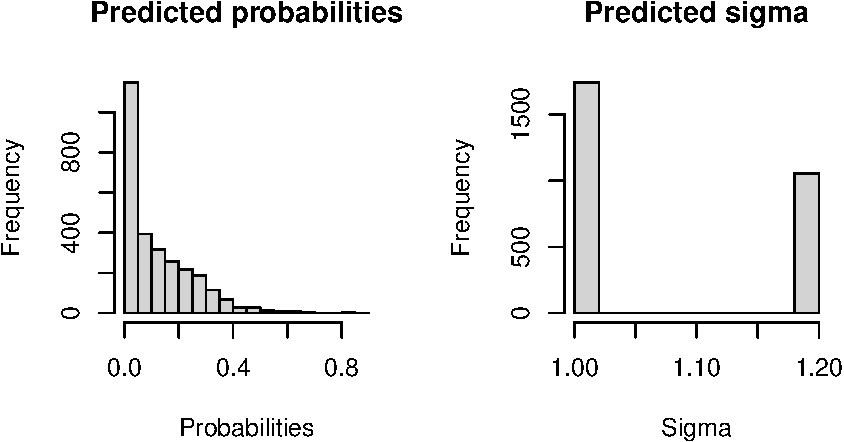
\includegraphics{RJ-2023-050_files/figure-latex/plothet-1.pdf}
\caption{\label{fig:plothet}Distribution of predicted probability and predicted sigma}
\end{figure}

An additional feature of \CRANpkg{Rchoice} package is that it allows to estimate the APEs for heteroskedastic binary models, as in Equation \eqref{eq:apehethat}, using \texttt{effect()} function. Similarly to command \texttt{margins()} from \CRANpkg{margins} package (Leeper 2021) or \texttt{avg\_slopes()} from \CRANpkg{marginaleffects} package (Arel-Bundock 2023), this function takes into account whether the variables are continuous, categorical or both. The user must specify categorical variables using \texttt{factor()} in the \texttt{formula} argument; otherwise, the \texttt{effect()} function will assume that the variable is continuous, when the variable may already be a \texttt{factor} in the dataset. In the following lines, we compute the APEs for a HET-Probit and HET-Logit model.\footnote{The Jacobian matrix is computed numerically using \texttt{jacobian()} function from \CRANpkg{numDeriv} package (Gilbert and Varadhan 2019).} The results are the following:

\begin{verbatim}
eff_logit  <- effect(het_logit2)
het_probit <- hetprob(tenure ~ factor(female) + year + I(year^2) + select +  
                        articles + prestige + factor(female)*articles | 
                        factor(female),              
                      data = sub_data,                        
                      link = "probit")
eff_probit <- effect(het_probit)
mtable(eff_probit,
       eff_logit)
\end{verbatim}

\begin{verbatim}
#> 
#> Calls:
#> eff_probit: hetprob(formula = tenure ~ factor(female) + year + I(year^2) + 
#>     select + articles + prestige + factor(female) * articles | 
#>     factor(female), data = sub_data, link = "probit", method = "nr")
#> eff_logit: hetprob(formula = tenure ~ factor(female) + year + I(year^2) + 
#>     select + articles + prestige + factor(female) * articles | 
#>     factor(female), data = sub_data, link = "logit", method = "nr")
#> 
#> =============================================
#>                    eff_probit    eff_logit   
#> ---------------------------------------------
#>   factor(female)1    -0.031**     -0.031**   
#>                      (0.012)      (0.012)    
#>   year                0.032***     0.032***  
#>                      (0.002)      (0.002)    
#>   select              0.014***     0.015***  
#>                      (0.004)      (0.004)    
#>   articles            0.006***     0.005***  
#>                      (0.001)      (0.001)    
#>   prestige           -0.035***    -0.036***  
#>                      (0.008)      (0.008)    
#> ---------------------------------------------
#>   Log-likelihood   -832.478     -835.133     
#>   N                2797         2797         
#> =============================================
#>   Significance: *** = p < 0.001;   
#>                 ** = p < 0.01; * = p < 0.05
\end{verbatim}

The APEs are very close to each other and statistically significant. According to the HET-Probit estimates, one additional published article increases the probability of being promoted by 0.6 percent points, whereas being a woman decreases the probability of promoted by 3.1\%.

\hypertarget{labor-participation}{%
\subsubsection{Labor participation}\label{labor-participation}}

Our second example is a replication of Greene (2003)`s example 17.7 based on the dataset ``\texttt{mroz.cvs}''. This dataset is based on a cross-section data on the wages of 428 working, married women, originating from the 1976 Panel Study of Income Dynamics (PSID), which can be loaded as follows:

\begin{verbatim}
mroz <- read.csv(file = 'mroz.csv')
mroz$kids <- with(mroz, factor((kidslt6 + kidsge6) > 0,
                               levels = c(FALSE, TRUE), 
                               labels = c("no", "yes")))
mroz$finc <-  mroz$faminc / 10000
\end{verbatim}

Using this data, Greene (2003) estimates the following HET-Probit model for women labor participation:
\begin{align}
\text{inlf}^* & = \beta_0 + \beta_1\text{age}+\beta_2\text{age}^2 + \beta_3\text{finc} + \beta_4\text{educ} + \beta_5\text{kids} + \epsilon, \label{eq:lfphet1} \\
\epsilon & \sim N(0, \sigma_i^2), \\
\sigma_i & = \exp(\delta_1 \text{kids} + \delta_2 \text{finc}),
\label{eq:lfphet2}
\end{align}
where \texttt{inlf} is a dummy variable indicating whether the woman participates in labor force, \texttt{age} is age in year, \texttt{finc} is family income in 1975 dollars divided by 10,000, \texttt{educ} is education in year and \texttt{kids} indicates whether children under 18 are present in the household. It is further assumed that \texttt{kids} and \texttt{finc} affect the variability of the error term.

The probit, Het-Probit and average marginal effects are estimated as follows:\footnote{Greene (2003) computes the marginal effects at the mean instead of the average marginal effects.}

\begin{verbatim}
labor_hom <- glm(inlf ~  age + I(age^2) + finc + educ + factor(kids), 
                 data = mroz, 
                 family = binomial(link = "probit"))
labor_het <- hetprob(inlf ~  age + I(age^2) + finc + educ + factor(kids) | 
                       factor(kids) + finc,              
                     data = mroz,                        
                     link = "probit")
eff_labor_het <- effect(labor_het)
mtable(labor_hom,
       labor_het,
       eff_labor_het)
\end{verbatim}

\begin{verbatim}
#> 
#> Calls:
#> labor_hom: glm(formula = inlf ~ age + I(age^2) + finc + educ + factor(kids), 
#>     family = binomial(link = "probit"), data = mroz)
#> labor_het: hetprob(formula = inlf ~ age + I(age^2) + finc + educ + factor(kids) | 
#>     factor(kids) + finc, data = mroz, link = "probit", method = "nr")
#> eff_labor_het: hetprob(formula = inlf ~ age + I(age^2) + finc + educ + factor(kids) | 
#>     factor(kids) + finc, data = mroz, link = "probit", method = "nr")
#> 
#> ========================================================================
#>                          labor_hom       labor_het       eff_labor_het  
#>                         -----------  ------------------   -----------   
#>                            inlf         mean    lnsigma      inlf       
#> ------------------------------------------------------------------------
#>   (Intercept)             -4.157**     -6.030*                          
#>                           (1.404)      (2.498)                          
#>   age                      0.185**      0.264*              -0.009***   
#>                           (0.066)      (0.118)              (0.003)     
#>   I(age^2)                -0.002**     -0.004*                          
#>                           (0.001)      (0.001)                          
#>   finc                     0.046        0.424    0.313*      0.069**    
#>                           (0.043)      (0.222)  (0.123)     (0.024)     
#>   educ                     0.098***     0.140**              0.030***   
#>                           (0.023)      (0.052)              (0.009)     
#>   factor(kids): yes/no    -0.449***    -0.879** -0.141      -0.161***   
#>                           (0.130)      (0.303)  (0.324)     (0.043)     
#> ------------------------------------------------------------------------
#>   Log-likelihood        -490.848     -487.636             -487.636      
#>   N                      753          753                  753          
#> ========================================================================
#>   Significance: *** = p < 0.001; ** = p < 0.01; * = p < 0.05
\end{verbatim}

The results show that family income does not play any role in the choice equation. However, it increases the variability of the error term. APE indicates that an increase of \$10,000 of family income increases the probability of labor force involvement by 6.9\%. There is not enough statistical evidence that proves having children under 18 in the household produces heteroskedasticity.

We can also use the Wald test provided by \texttt{linearHypothesis()} function from \CRANpkg{car} package to test the null hypothesis of homoskedasticity:

\begin{verbatim}
coefs <- names(coef(labor_het))
linearHypothesis(labor_het, coefs[grep("het", coefs)])
\end{verbatim}

\begin{verbatim}
#> Linear hypothesis test
#> 
#> Hypothesis:
#> het.factor(kids)yes = 0
#> het.finc = 0
#> 
#> Model 1: restricted model
#> Model 2: inlf ~ age + I(age^2) + finc + educ + factor(kids) | factor(kids) + 
#>     finc
#> 
#>   Df  Chisq Pr(>Chisq)  
#> 1                       
#> 2  2 6.5331    0.03814 *
#> ---
#> Signif. codes:  0 '***' 0.001 '**' 0.01 '*' 0.05 '.' 0.1 ' ' 1
\end{verbatim}

The null hypothesis of homoskedasticity is rejected at the 5\% with a \(\chi_2^2 = 6.533\).

Supplementary materials provide Stata code (version 16.1) to replicate all the results in this Section. The log file is presented in \textbf{Appendix C}. Overall, the results using Stata are exactly the same to those reported by \texttt{hetprob()} function from \CRANpkg{Rchoice} package.

\hypertarget{instrumental-variable-probit-model}{%
\subsection{Instrumental variable probit model}\label{instrumental-variable-probit-model}}

\hypertarget{control-function-approach}{%
\subsubsection{Control function approach}\label{control-function-approach}}

In this example, and similar to Wooldridge (2010), we use the \texttt{mroz} sample and assume the following slightly modified model for married women's labor force participation from previous Section:
\begin{align*}
  \text{inlf}^* = &  \beta_0 + \beta_1\text{educ} + \beta_2 \text{exper} + \beta_3\text{exper}^2+\beta_4\text{age}+\beta_5 \text{kidslt6} +\\
                    &  \beta_6 \text{kidsge6}+\beta_7\text{nwifeinc}+ \epsilon, \\
  \text{nwifeinc} = & \delta_0 + \delta_1\text{educ} + \delta_2 \text{exper} + \delta_3\text{exper}^2+\delta_4\text{age}+\delta_5 \text{kidslt6} +\\
                    &  \delta_6 \text{kidsge6}+\delta_7\text{huseduc}+ \upsilon, \\          \text{lfp}   & =  \mathbf{1}\left[\text{lfp}^* > 0\right]
\end{align*}
where \texttt{nwifeinc} is the other sources of income (divided by 1,000) and assumed to be endogenous. A just identified IV model is estimated by using husband's education, (\texttt{huseduc}), as an instrument for \texttt{nwifeinc}. The strong identification assumption here is that husband's schooling is unrelated to factors that affect a married woman's labor force decision once \texttt{nwifeinc} and the other variables are accounted for (Wooldridge 2010).

When interpreting the results from an IV model, it is important to compare its magnitude with a model that assumes exogeneity. In this example, our benchmark APE for \texttt{nwifeinc} is obtained by the standard probit model:

\begin{verbatim}
probit <- glm(inlf ~  educ + exper + I(exper^2) + age + kidslt6 + kidsge6 + nwifeinc, 
              data = mroz, 
              family = binomial(link = "probit"))
ape.probit <- mean(dnorm(predict(probit, type = "link"))) * coef(probit)["nwifeinc"]
ape.probit
\end{verbatim}

\begin{verbatim}
#>     nwifeinc 
#> -0.003616176
\end{verbatim}

Accordingly, an increase of \$1,000 in other sources of income reduces the labor force participation probability by 0.4\%, holding all other factors constant. Note that the same APE, along with its standard error, can also be obtained using \texttt{avg\_slopes()} command:

\begin{verbatim}
library("marginaleffects")
avg_slopes(probit, variables = "nwifeinc")
\end{verbatim}

\begin{verbatim}
#> 
#>      Term Estimate Std. Error     z Pr(>|z|)   S   2.5 %    97.5 %
#>  nwifeinc -0.00362    0.00147 -2.46   0.0139 6.2 -0.0065 -0.000736
#> 
#> Columns: term, estimate, std.error, statistic, p.value, s.value, conf.low, conf.high 
#> Type:  response
\end{verbatim}

I proceed to estimate the model using the CF approach. First, I estimate the first-step equation, which is a linear model, and obtain the residuals \(\widetilde{\upsilon}\):

\begin{verbatim}
fstep   <- lm(nwifeinc ~ educ + exper + I(exper^2) + age + kidslt6 + kidsge6  + huseduc, 
            data = mroz)
mroz$res.hat <- fstep$residuals
\end{verbatim}

We can also test the power of the instrument using \texttt{linearHypothesis()} function:

\begin{verbatim}
linearHypothesis(fstep, "huseduc")
\end{verbatim}

\begin{verbatim}
#> Linear hypothesis test
#> 
#> Hypothesis:
#> huseduc = 0
#> 
#> Model 1: restricted model
#> Model 2: nwifeinc ~ educ + exper + I(exper^2) + age + kidslt6 + kidsge6 + 
#>     huseduc
#> 
#>   Res.Df   RSS Df Sum of Sq      F    Pr(>F)    
#> 1    746 86955                                  
#> 2    745 81120  1    5834.8 53.586 6.427e-13 ***
#> ---
#> Signif. codes:  0 '***' 0.001 '**' 0.01 '*' 0.05 '.' 0.1 ' ' 1
\end{verbatim}

The first-stage \(F\) statistic on \texttt{huseduc} is substantially above the traditional cut-off of ten suggesting that the instrument is not weak.

The second-step is computed using \texttt{glm()} function and adding the residuals (\texttt{res.hat}) as an additional explanatory variable:

\begin{verbatim}
sstep   <- glm(inlf ~  educ + exper + I(exper^2) + age + kidslt6 + kidsge6 + nwifeinc + res.hat, 
            data   = mroz, 
            family = binomial(link = "probit")) 
summary(sstep)
\end{verbatim}

\begin{verbatim}
#> 
#> Call:
#> glm(formula = inlf ~ educ + exper + I(exper^2) + age + kidslt6 + 
#>     kidsge6 + nwifeinc + res.hat, family = binomial(link = "probit"), 
#>     data = mroz)
#> 
#> Deviance Residuals: 
#>     Min       1Q   Median       3Q      Max  
#> -2.2523  -0.9078   0.4204   0.8566   2.2803  
#> 
#> Coefficients:
#>               Estimate Std. Error z value Pr(>|z|)    
#> (Intercept)  0.0171183  0.5380339   0.032  0.97462    
#> educ         0.1702142  0.0377615   4.508 6.56e-06 ***
#> exper        0.1163118  0.0193869   6.000 1.98e-09 ***
#> I(exper^2)  -0.0019458  0.0005999  -3.244  0.00118 ** 
#> age         -0.0449529  0.0101351  -4.435 9.19e-06 ***
#> kidslt6     -0.8444319  0.1197268  -7.053 1.75e-12 ***
#> kidsge6      0.0477912  0.0449431   1.063  0.28761    
#> nwifeinc    -0.0368639  0.0183848  -2.005  0.04495 *  
#> res.hat      0.0267092  0.0191539   1.394  0.16318    
#> ---
#> Signif. codes:  0 '***' 0.001 '**' 0.01 '*' 0.05 '.' 0.1 ' ' 1
#> 
#> (Dispersion parameter for binomial family taken to be 1)
#> 
#>     Null deviance: 1029.75  on 752  degrees of freedom
#> Residual deviance:  800.61  on 744  degrees of freedom
#> AIC: 818.61
#> 
#> Number of Fisher Scoring iterations: 4
\end{verbatim}

Since the \(z\)-statistic for \texttt{res.hat} is 1.4, we cannot reject the null hypothesis that \texttt{nwifeinc} is exogenous: \(H_0:\lambda = 0\).

An estimate of \(\rho\) can be obtained using Equation \eqref{eq:estimaterho} and the following syntax:

\begin{verbatim}
lambda.hat    <- coef(sstep)["res.hat"]
k             <- length(fstep$coefficients)
SSE           <- sum(fstep$residuals^2)
n             <- length(fstep$residuals)
sigma.upsilon <- sqrt(SSE/(n - k))
rho.hat       <- lambda.hat * sigma.upsilon
rho.hat
\end{verbatim}

\begin{verbatim}
#>   res.hat 
#> 0.2787068
\end{verbatim}

Thus, the estimated correlation using the CF approach is \(\widehat{\rho} = 0.279\). It is important to recall that the estimated coefficients for the \texttt{sstep} model represent the coefficients scaled by a factor of \(1 / \sqrt{1 - \rho^2}\). Moreover, the standard errors from the \texttt{sstep} model are biased since they do not consider the sampling error of the first stage. However, we can use \texttt{ivprobit()} function from \CRANpkg{ivprobit} package (Zaghdoudi 2018) to get the correct standard errors:\footnote{\texttt{ivprobit()} uses a minimum chi-squared estimator (Newey 1987).}

\begin{verbatim}
library("ivprobit")
twostep.probit <- ivprobit(inlf ~  educ + exper + I(exper^2) + age + kidslt6 + kidsge6 | 
                             nwifeinc | educ + exper + I(exper^2) + age + kidslt6 + 
                             kidsge6 + huseduc, 
                           data = mroz)
summary(twostep.probit)
\end{verbatim}

\begin{verbatim}
#>                   Coef        S.E.  t-stat     p-val    
#> Intercep    0.01711834  0.54865782  0.0312  0.975118    
#> educ        0.17021419  0.03848938  4.4224 1.121e-05 ***
#> exper       0.11631183  0.01976301  5.8853 6.001e-09 ***
#> I(exper^2) -0.00194584  0.00061195 -3.1798  0.001535 ** 
#> age        -0.04495285  0.01032548 -4.3536 1.526e-05 ***
#> kidslt6    -0.84443188  0.12176581 -6.9349 8.818e-12 ***
#> kidsge6     0.04779117  0.04578807  1.0437  0.296940    
#> nwifeinc   -0.03686390  0.01874338 -1.9668  0.049580 *  
#> ---
#> Signif. codes:  0 '***' 0.001 '**' 0.01 '*' 0.05 '.' 0.1 ' ' 1
\end{verbatim}

The estimates of the \texttt{sstep} and \texttt{twostep.probit} models are the same, while their standard errors are slightly different.

The APE for \texttt{nwifeinc}---and any other continuous variable---can be computed using Equation \eqref{eq:apey2cf} and its standard error via bootstrap method. Below, I use package \CRANpkg{boot} (Canty 2002) to perform the simulation. First, a function called \texttt{ape()} is created which returns the APE. The first argument of this function is the dataset, whereas the second argument can be an index vector of the observations in the dataset.

\begin{verbatim}
ape <- function(data, indices){
  d <- data[indices, ]
  # Compute the first-stage regression
  fstep    <- lm(nwifeinc ~ educ + exper + I(exper^2) + age + kidslt6 + kidsge6 + 
                   huseduc, 
                 data = d)
  # Obtain the residuals 
  d$res.hat <- fstep$residuals
  # Compute the second-stage regression
  sstep   <- glm(inlf ~  educ + exper + I(exper^2) + age + kidslt6 + kidsge6 + 
                   nwifeinc + res.hat, 
                 data   = d, 
                 family = binomial(link = "probit"))
  # Compute APE for nwincome
  out <- mean(dnorm(predict(sstep, type = "link"))) * coef(sstep)["nwifeinc"]
  return(out)
}
\end{verbatim}

Once we have defined the function \texttt{ape()}, we can use the \texttt{boot()} function to perform the bootstrap procedure. In the following syntax, \texttt{R\ =\ 500} resamplings are used and the 90\%-CI interval is obtained using \texttt{boot.ci()} function.

\begin{verbatim}
library("boot")
set.seed(666)
results <- boot(data = mroz, statistic = ape, R = 500)
results
\end{verbatim}

\begin{verbatim}
#> 
#> ORDINARY NONPARAMETRIC BOOTSTRAP
#> 
#> 
#> Call:
#> boot(data = mroz, statistic = ape, R = 500)
#> 
#> 
#> Bootstrap Statistics :
#>       original        bias    std. error
#> t1* -0.0110576 -0.0005050597 0.005877061
\end{verbatim}

\begin{verbatim}
boot.ci(results, type = "norm", conf = 0.90)
\end{verbatim}

\begin{verbatim}
#> BOOTSTRAP CONFIDENCE INTERVAL CALCULATIONS
#> Based on 500 bootstrap replicates
#> 
#> CALL : 
#> boot.ci(boot.out = results, conf = 0.9, type = "norm")
#> 
#> Intervals : 
#> Level      Normal        
#> 90%   (-0.0202, -0.0009 )  
#> Calculations and Intervals on Original Scale
\end{verbatim}

The results show that another \$1,000 in other sources of income reduces the labor force participation probability by 1.1 percent points with 90\%-CI \(\left[-2, -.09\right]\). This estimate, which is marginally statistically significant, is about three times larger than the probit estimate that treats \texttt{nwifeinc} as exogenous: \texttt{-0.04}.

Finally, we can recover the unscaled parameters by multiplying the coefficients by \(\sqrt{\left(1 - \widehat{\rho}^2\right)}\) as follows:

\begin{verbatim}
coef(sstep) * sqrt(1 - rho.hat^2)
\end{verbatim}

\begin{verbatim}
#>  (Intercept)         educ        exper   I(exper^2)          age      kidslt6 
#>  0.016440046  0.163469667  0.111703116 -0.001868741 -0.043171653 -0.810972324 
#>      kidsge6     nwifeinc      res.hat 
#>  0.045897507 -0.035403215  0.025650873
\end{verbatim}

\hypertarget{maximum-likelihood-estimator}{%
\subsubsection{Maximum likelihood estimator}\label{maximum-likelihood-estimator}}

In this Section I estimate the model from previous Section using the MLE. To do so, I use the \texttt{ivpml()} function from \CRANpkg{Rchoice} package. The syntax is as follows:

\begin{verbatim}
fiml.probit <- ivpml(inlf ~  educ + exper + I(exper^2) + age + kidslt6 + kidsge6 + 
                       nwifeinc | huseduc +  educ + exper + I(exper^2) + age + 
                       kidslt6 + kidsge6, 
                     data = mroz)
\end{verbatim}

\begin{verbatim}
#> 
#> Estimating a just identified model....
#> 
#> Obtaining starting values from probit and linear model...
\end{verbatim}

The syntax of \texttt{ivpml()} is similar to that of \texttt{ivreg()} function from \CRANpkg{AER} package. The \texttt{formula} has two part in the right-hand side, that is, \texttt{y\ \textasciitilde{}\ x\ \textbar{}\ z} where \texttt{y} is the binary response variable, \texttt{x} are the regressors (\(\mathbf x\) in Equation \eqref{eq:firsteq}), and \texttt{z} are the exogenous variables (\(\mathbf x_1\) and \(\mathbf x_2\) in Equation \eqref{eq:secondeq}).

During the optimization procedure, \texttt{ivpml()} displays several messages which can be turned-off by setting \texttt{messages\ =\ FALSE}. The output indicates that the model is just-identified and that the initial values for the optimization procedure are obtained from the traditional probit and linear models for the structural and first-stage equation, respectively. Similarly to \texttt{hetprob()} function, the optimization algorithm can be managed using the argument \texttt{method}, which is passed on to the \texttt{maxLik()} function. Currently, the default algorithm is the Newton-Raphson, \texttt{method\ =\ "nr"}.

\begin{verbatim}
summary(fiml.probit)
\end{verbatim}

\begin{verbatim}
#> --------------------------------------------
#> Maximum Likelihood estimation of IV Probit model 
#> Newton-Raphson maximisation, 3 iterations
#> Return code 8: successive function values within relative tolerance limit (reltol)
#> Log-Likelihood: -3230.642 
#> 18  free parameters
#> Estimates:
#>                         Estimate  Std. error z value   Pr(> z)    
#> inlf:(Intercept)      1.6499e-02  5.3008e-01  0.0311 0.9751702    
#> inlf:educ             1.6403e-01  3.1225e-02  5.2531 1.495e-07 ***
#> inlf:exper            1.1209e-01  2.1199e-02  5.2873 1.241e-07 ***
#> inlf:I(exper^2)      -1.8751e-03  5.9150e-04 -3.1701 0.0015237 ** 
#> inlf:age             -4.3319e-02  1.1331e-02 -3.8230 0.0001319 ***
#> inlf:kidslt6         -8.1375e-01  1.2994e-01 -6.2623 3.794e-10 ***
#> inlf:kidsge6          4.6054e-02  4.3139e-02  1.0676 0.2857141    
#> inlf:nwifeinc        -3.5524e-02  1.6190e-02 -2.1941 0.0282247 *  
#> nwifeinc:(Intercept) -1.4720e+01  3.7672e+00 -3.9076 9.322e-05 ***
#> nwifeinc:huseduc      1.1782e+00  1.6009e-01  7.3594 1.847e-13 ***
#> nwifeinc:educ         6.7469e-01  2.1254e-01  3.1744 0.0015016 ** 
#> nwifeinc:exper       -3.1299e-01  1.3752e-01 -2.2760 0.0228480 *  
#> nwifeinc:I(exper^2)  -4.7756e-04  4.4955e-03 -0.1062 0.9153983    
#> nwifeinc:age          3.4015e-01  5.9390e-02  5.7274 1.020e-08 ***
#> nwifeinc:kidslt6      8.2627e-01  8.1402e-01  1.0151 0.3100812    
#> nwifeinc:kidsge6      4.3553e-01  3.2027e-01  1.3599 0.1738728    
#> lnsigma               2.3398e+00  2.5768e-02 90.8016 < 2.2e-16 ***
#> atanhrho              2.7379e-01  1.9296e-01  1.4189 0.1559361    
#> ---
#> Signif. codes:  0 '***' 0.001 '**' 0.01 '*' 0.05 '.' 0.1 ' ' 1
#> 
#> Instrumented: nwifeinc
#> Instruments: (Intercept) huseduc educ exper I(exper^2) age kidslt6 kidsge6 
#> Wald test of exogeneity (corr = 0): chi2 2.01 with 1 df. Prob > chi2 =  0.1559 
#> --------------------------------------------
\end{verbatim}

During the optimization procedure the parameters \(\sigma_{\upsilon}\) and \(\rho\) might tend to the boundary points of the parameter space, generating identifiability problems of the MLE. To avoid this issue, \texttt{ivpml()} re-parametrizes the parameters.\footnote{This re-parametrization is also used by \texttt{ivprobit} function in Stata.} First, to ensure \(\sigma_{\upsilon} > 0\), \texttt{ivpml()} instead estimates \(\log \nu_{\upsilon}\) such that:
\begin{equation}
\sigma_{\upsilon} = \exp(\log \nu_{\upsilon}). 
  \label{eq:repsigma}
\end{equation}

Second, \texttt{ivpml()} forces the correlation to remain in the \((-1, +1)\) range by using the inverse hyperbolic tangent:
\begin{equation*}
\textrm{atanh}(\rho) = \tau = \frac{1}{2}\log\left(\frac{1 +  \rho}{1 - \rho}\right),
\end{equation*}
where \(\tau\) is unrestricted, and \(\rho\) can be obtained using the inverse of \(\tau\):
\begin{equation}
\tau ^{-1} = \rho = \tanh(\tau).
  \label{eq:reprho}
\end{equation}

In the following syntax, we recover \(\sigma_{\upsilon}\) and \(\rho\) using Equations \eqref{eq:repsigma} and \eqref{eq:reprho}, respectively, and their standard errors are computed using delta method approach by \texttt{deltaMethod()} function:

\begin{verbatim}
deltaMethod(fiml.probit, "exp(lnsigma)")
\end{verbatim}

\begin{verbatim}
#>              Estimate       SE    2.5 % 97.5 %
#> exp(lnsigma) 10.37928  0.26746  9.85508 10.903
\end{verbatim}

\begin{verbatim}
deltaMethod(fiml.probit, "tanh(atanhrho)")
\end{verbatim}

\begin{verbatim}
#>                 Estimate        SE     2.5 % 97.5 %
#> tanh(atanhrho)  0.267145  0.179190 -0.084061 0.6184
\end{verbatim}

Again, the FIML estimate of \(\rho\) is close to that found using the CF approach which was \texttt{0.279}. If significant, a positive \(\rho\) would indicate that there is a positive correlation between \(\epsilon\) and \(\upsilon\). That is, the unobserved factors that make it more likely for a woman to have a higher income from other sources also make it more likely that the woman will be participating in the labor force.

For those users who are more familiar with Stata (see \textbf{Appendix D}), it is important to mention that its function \texttt{ivprobit} estimates the 95\%-CI for \(\widehat{\rho}\) and \(\widehat{\sigma}_{\upsilon}\) as follows:

\begin{verbatim}
cbind(exp(coef(fiml.probit)["lnsigma"] - qnorm(0.975) * stdEr(fiml.probit)["lnsigma"]), 
      exp(coef(fiml.probit)["lnsigma"] + qnorm(0.975) * stdEr(fiml.probit)["lnsigma"]))
\end{verbatim}

\begin{verbatim}
#>             [,1]     [,2]
#> lnsigma 9.868094 10.91695
\end{verbatim}

\begin{verbatim}
cbind(tanh(coef(fiml.probit)["atanhrho"] - qnorm(0.975) * stdEr(fiml.probit)["atanhrho"]), 
      tanh(coef(fiml.probit)["atanhrho"] + qnorm(0.975) * stdEr(fiml.probit)["atanhrho"]))
\end{verbatim}

\begin{verbatim}
#>                [,1]      [,2]
#> atanhrho -0.1040317 0.5730038
\end{verbatim}

The APEs can be estimated using the function \texttt{effect()}. The main argument of this function is \texttt{asf}. If \texttt{asf\ =\ TRUE} (the default), then the APEs are computed using Equation \eqref{eq:ME1y2ivprobit}. On the other hand, if \texttt{asf\ =\ FALSE} the APEs are computed using Equation \eqref{eq:ME2y2ivprobit}.

\begin{verbatim}
summary(effect(fiml.probit))
\end{verbatim}

\begin{verbatim}
#> ------------------------------------------------------
#> Marginal effects for the IV Probit model:
#> ------------------------------------------------------
#>               dydx Std. error z value  Pr(> z)    
#> educ      0.051057   0.011101   4.599 4.24e-06 ***
#> exper     0.023071   0.002952   7.816 5.44e-15 ***
#> age      -0.013484   0.002986  -4.516 6.31e-06 ***
#> kidslt6  -0.253295   0.033077  -7.658 1.89e-14 ***
#> kidsge6   0.014335   0.013520   1.060   0.2890    
#> nwifeinc -0.011058   0.005550  -1.992   0.0463 *  
#> ---
#> Signif. codes:  0 '***' 0.001 '**' 0.01 '*' 0.05 '.' 0.1 ' ' 1
#> 
#> Note: Marginal effects computed as the average for each individual
\end{verbatim}

\begin{verbatim}
summary(effect(fiml.probit, asf = FALSE))
\end{verbatim}

\begin{verbatim}
#> ------------------------------------------------------
#> Marginal effects for the IV Probit model:
#> ------------------------------------------------------
#>               dydx Std. error z value  Pr(> z)    
#> educ      0.048777   0.008733   5.585 2.33e-08 ***
#> exper     0.021997   0.003723   5.908 3.46e-09 ***
#> age      -0.012882   0.003322  -3.878 0.000105 ***
#> kidslt6  -0.241982   0.036594  -6.613 3.78e-11 ***
#> kidsge6   0.013695   0.012792   1.071 0.284373    
#> nwifeinc -0.010564   0.004736  -2.230 0.025724 *  
#> ---
#> Signif. codes:  0 '***' 0.001 '**' 0.01 '*' 0.05 '.' 0.1 ' ' 1
#> 
#> Note: Marginal effects computed as the average for each individual
\end{verbatim}

The results show that both APEs are close to each other. Note also that the estimated APE for \texttt{nwifeinc} using the CF approach is very similar to that ones obtained by MLE. \textbf{Appendix D} also shows that the Stata function \texttt{ivprobit()} provides the same estimates and marginal effects as \texttt{ivpml()} function.

\hypertarget{summary}{%
\section{Summary}\label{summary}}

The aim of the article was to provide a primer on estimating heteroskedastic and IV model for binary outcomes in R. I also show that the current version of \CRANpkg{Rchoice} package (available at \url{https://cran.r-project.org/web/packages/Rchoice/index.html}) allows to estimate such models in a flexible way and provides accurate average marginal effects that are very similar to those provided by Stata's \code{margins} command. \CRANpkg{Rchoice} can be used in concert with other packages. For example, one can format the summary output from \CRANpkg{Rchoice} with \CRANpkg{memisc} to produce well-formatted tables for regression estimates

\hypertarget{appendix-a-gradient-and-hessian-for-binary-response-models-with-heteroskedasticity}{%
\section{Appendix A: Gradient and Hessian for binary response models with heteroskedasticity}\label{appendix-a-gradient-and-hessian-for-binary-response-models-with-heteroskedasticity}}

In this section, I provide the analytic gradient and Hessian used by \texttt{hetprob()} function in \CRANpkg{Rchoice}. The log-likelihood function for the binary choice model with exponential heteroskedasticity can be written as:
\begin{equation*}
\ell(\boldsymbol \theta)= \sum_{i = 1}^n\ln F(a_i),
\end{equation*}
where \(F(\cdot)\) is either the CDF of the standard normal or standard logistic distribution, \(\boldsymbol \theta= \left(\boldsymbol \beta^\top, \boldsymbol \delta^\top\right)^\top\) is the full \((k+p)\)-dimensional vector of parameters, and:
\begin{equation*}
\begin{aligned}
a_i & = q_i\left(\frac{\mathbf x_i^\top\boldsymbol \beta}{\exp(\mathbf z_i^\top\boldsymbol \delta)}\right), \\
q_i & = 2(y_{i}-1).
\end{aligned}
\end{equation*}

The gradient is:
\begin{equation*}
\begin{aligned}
\frac{\partial \ell(\boldsymbol \theta)}{\partial \boldsymbol \theta} & = \sum_{i=1}^n\left[\frac{f(a_i)}{F(a_i)}\frac{\partial a_i}{\partial \boldsymbol \theta}\right], \\
& = \sum_{i=1}^n\left[m(a_i)\mathbf g_{i}\right],
\end{aligned}
\end{equation*}
where \(m(\cdot)=f(\cdot)/F(\cdot)=\phi(\cdot)/\Phi(\cdot)\) for the probit model and \(m(\cdot) = 1 - \Lambda(\cdot)\) for the logit model, and \(\partial a_i/\partial \boldsymbol \theta= \mathbf g_i\) such that:
\begin{equation*}
\mathbf g_{i}  = \begin{pmatrix}
                      \frac{\partial a_i}{\partial \boldsymbol \beta} \\
                      \frac{\partial a_i}{\partial \boldsymbol \delta}
                     \end{pmatrix}
                   = \frac{q_i}{\exp(\mathbf z_i^\top\boldsymbol \delta)}
                     \begin{pmatrix}
                      \mathbf x_i \\
                      -\left(\mathbf x_i^\top\boldsymbol \beta\right)\mathbf z_i
                     \end{pmatrix}.
\end{equation*}

The Hessian is given by:
\begin{equation*}
\begin{aligned}
\frac{\partial^2 \ell(\boldsymbol \theta)}{\partial \boldsymbol \theta\partial \boldsymbol \theta^\top}& = \frac{\partial }{\partial \boldsymbol \theta^\top}\left(\frac{\partial \ell(\boldsymbol \theta)}{\partial \boldsymbol \theta} \right), \\
& = \sum_{i = 1}^n\left[h(a_i)\mathbf g_{i}\mathbf g_{i}^\top + m(a_i)\mathbf H_{i}\right],
\end{aligned}
\end{equation*}
where \(h(a_i) = \partial m(a_i)/\partial a_i=-a_im(a_i)-m(a_i)^2\) and:
\begin{equation*}
\mathbf H_i = \frac{\partial a_i}{\partial \boldsymbol \theta\partial \boldsymbol \theta^\top} = \begin{pmatrix}
\frac{\partial a_i}{\partial \boldsymbol \beta\partial \boldsymbol \beta^\top} & \frac{\partial a_i}{\partial \boldsymbol \beta\partial \boldsymbol \delta^\top} \\
\frac{\partial a_i}{\partial \boldsymbol \delta\partial \boldsymbol \beta^\top} &  \frac{\partial a_i}{\partial \boldsymbol \delta\partial \boldsymbol \delta^\top}
\end{pmatrix}
=
\begin{pmatrix}
  \mathbf O& -\frac{q_i}{\exp(\mathbf z_i^\top\boldsymbol \delta)}\mathbf x_i\mathbf z_i^\top \\
  -\frac{q_i}{\exp(\mathbf z_i^\top\boldsymbol \delta)}\mathbf z_i\mathbf x_i^\top & \frac{q_i(\mathbf x_i^\top\boldsymbol \beta)}{\exp(\mathbf z_i^\top\boldsymbol \delta)}\mathbf z_i\mathbf z_i^\top
\end{pmatrix}.
\end{equation*}

\hypertarget{appendix-b-gradient-and-hessian-for-binary-response-models-with-endogeneity}{%
\section{Appendix B: Gradient and Hessian for binary response models with endogeneity}\label{appendix-b-gradient-and-hessian-for-binary-response-models-with-endogeneity}}

In this section, I provide the analytic gradient and Hessian used by \code{ivpml} function in \CRANpkg{Rchoice}. The log-likelihood function can be written as:
\begin{equation*}
\ell(\boldsymbol \theta) = \sum_{i = 1}^n\left[\ln\left(\Phi(a_i)\right)+\ln(1)-\ln\left(\sigma_{\upsilon}\right)+\ln\left[\phi(b_i)\right]\right],
\end{equation*}
where \(\boldsymbol \theta= \left(\boldsymbol \beta^\top, \boldsymbol \delta^\top, \sigma_{\upsilon}, \rho\right)^\top\) is an \((k + p + 2)\)-dimensional vector and:
\begin{equation*}
\begin{aligned}
  a_i & =  q_i\left(\frac{\mathbf x_i^\top\boldsymbol \beta+ \frac{\rho}{\sigma_{\upsilon}}\left(y_{2i}-\mathbf z_i^\top\boldsymbol \delta\right)}{\sqrt{1-\rho^2}}\right),\\
  b_i & = \frac{y_{2i}-\mathbf z_i^\top\boldsymbol \delta}{\sigma_{\upsilon}},\\
  q_i & = 2(y_i - 1),\\
  \sigma_{\upsilon} &= \exp(\ln \nu_{\upsilon}), \\
  \rho & = \text{tanh}(\tau). 
\end{aligned}
\end{equation*}

The first derivatives of the log-likelihood function are:
\begin{equation*}
\begin{aligned}
\frac{\partial \ell(\boldsymbol \theta)}{\partial \boldsymbol \beta} & = \sum_{i = 1}^n\left[m(a_i)\left(\frac{q_i}{\sqrt{1-\rho^2}}\right)\mathbf x_i\right], \\
\frac{\partial \ell(\boldsymbol \theta)}{\partial \boldsymbol \delta} & = \sum_{i = 1}^n\left[-m(a_i)\left(\frac{q_i\left(\rho/\sigma_{\upsilon}\right)}{\sqrt{1-\rho^2}}\right)+b_i\left(\frac{1}{\sigma_{\upsilon}}\right)\right]\mathbf z_i, \\
\frac{\partial \ell(\boldsymbol \theta)}{\partial \ln \nu_{\upsilon}} & = \sum_{i = 1}^n\left[-m(a_i)\frac{q_i\rho}{\sqrt{1-\rho^2}}b_i+b_i^2-1\right], \\
\frac{\partial \ell(\boldsymbol \theta)}{\partial \tau}
& = \sum_{i = 1}^n\left[m(a_i)q_i\left(\frac{\mathbf x_i^\top\boldsymbol \beta\rho +    b_i}{\sqrt{\text{sech}^2(\tau)}}\right)\right],
\end{aligned}
\end{equation*}
where \(m(a_i)=\phi(a_i)/\Phi(a_i)\), \(d\text{tanh}(\tau)/d\tau = \text{sech}^2(\tau)\), and we use the fact that \(\phi'(b_i)= -b_i\phi(b_i)\) so that \(\phi'(b_i)/\phi(b_i)=-b_i\).

The Hessian is given by:
\begin{equation*}
\mathbf H= \begin{pmatrix}
         \frac{\partial^2 \ell(\boldsymbol \theta)}{\partial \boldsymbol \beta\partial \boldsymbol \beta^\top} & \frac{\partial^2 \ell(\boldsymbol \theta)}{\partial \boldsymbol \beta\partial \boldsymbol \delta^\top} & \frac{\partial^2 \ell(\boldsymbol \theta)}{\partial \boldsymbol \beta\partial \ln \nu_{\upsilon}} & \frac{\partial^2 \ell(\boldsymbol \theta)}{\partial \boldsymbol \beta\partial \tau} \\
         \dot &  \frac{\partial^2 \ell(\boldsymbol \theta)}{\partial \boldsymbol \delta\partial \boldsymbol \delta^\top} &   \frac{\partial^2 \ell(\boldsymbol \theta)}{\partial \boldsymbol \delta\partial \partial \ln \nu_{\upsilon}} & \frac{\partial^2 \ell(\boldsymbol \theta)}{\partial \boldsymbol \delta\partial \tau} \\
         \dot & \dot & \frac{\partial^2 \ell(\boldsymbol \theta)}{\partial (\ln \nu_{\upsilon})^2} & \frac{\partial^2 \ell(\boldsymbol \theta)}{\partial \ln \nu_{\upsilon} \partial \tau} \\
         \dot & \dot & \dot & \frac{\partial^2 \ell(\boldsymbol \theta)}{\partial \tau^2}
      \end{pmatrix}.
\end{equation*}

The second derivatives are:
\begin{equation*}
\begin{aligned}
\frac{\partial^2 \ell(\boldsymbol \theta)}{\partial \boldsymbol \beta\partial \boldsymbol \beta^\top} & = \sum_{i = 1}^n\left[h(a_i)\left(\frac{q_i}{\sqrt{1-\rho^2}}\right)^2\mathbf x_i\mathbf x_i^\top\right],  \\
\frac{\partial^2 \ell(\boldsymbol \theta)}{\partial \boldsymbol \beta\partial \boldsymbol \delta^\top} & =\sum_{i = 1}^n\left[-h(a_i)\left(\frac{q_i}{\sqrt{1-\rho^2}}\right)^2\left(\frac{\rho}{\sigma_{\upsilon}}\right)\mathbf x_i\mathbf z_i^\top\right],  \\
\frac{\partial^2 \ell(\boldsymbol \theta)}{\partial \boldsymbol \beta\partial \ln \nu_{\upsilon}} & =\sum_{i = 1}^n\left[-h(a_i)\left(\frac{q_i}{\sqrt{1-\rho^2}}\right)^2\left(\rho b_i\right)\mathbf x_i\right],  \\
\frac{\partial^2 \ell(\boldsymbol \theta)}{\partial \boldsymbol \beta\partial \tau} & =\sum_{i = 1}^n\left[h(a_i)\left(\frac{q_i}{\sqrt{1-\rho^2}}\right)\left(q_i\left(\frac{\mathbf x_i^\top\boldsymbol \beta\rho +b_i}{\sqrt{\text{sech}^2(\tau)}}\right)\right)\mathbf x_i\right], \\
  \frac{\partial^2 \ell(\boldsymbol \theta)}{\partial \boldsymbol \delta\partial \boldsymbol \delta^\top} & = \sum_{i = 1}^n\left[h(a_i)\left(\frac{q_i\left(\rho/\sigma_{\upsilon}\right)}{\sqrt{1-\rho^2}}\right)^2-\frac{1}{\sigma^2_{\upsilon}}\right]\mathbf z_i\mathbf z_i^\top, \\
  \frac{\partial^2 \ell(\boldsymbol \theta)}{\partial \boldsymbol \delta\partial \ln \nu_{\upsilon}} & =\sum_{i = 1}^n\left(\frac{b_i}{\sigma_{\upsilon}}\right)\left[h(a_i)\left(\frac{q_i\rho}{\sqrt{1-\rho^2}}\right)^2-2\right]\mathbf z_i, \\
    \frac{\partial^2 \ell(\boldsymbol \theta)}{\partial \boldsymbol \delta\partial \tau} & =\sum_{i = 1}^n\left[-h(a_i)\left(\frac{q_i\left(\rho/\sigma_{\upsilon}\right)}{\sqrt{1-\rho^2}}\right)\left(q_i\left(\frac{\mathbf x_i^\top\boldsymbol \beta\rho +b_i}{\sqrt{\text{sech}^2(\tau)}}\right)\right)\right]\mathbf z_i, \\
\frac{\partial^2 \ell(\boldsymbol \theta)}{\partial (\ln \nu_{\upsilon})^2}& = \sum_{i = 1}^n\left[h(a_i)\left(\frac{q_i\rho b_i}{\sqrt{1-\rho^2}}\right)^2+m(a_i)\left(\frac{q_i\rho b_i}{\sqrt{1-\rho^2}}\right)-2b_i^2\right], \\
\frac{\partial^2 \ell(\boldsymbol \theta)}{\partial \ln \nu_{\upsilon} \partial \tau} & = \sum_{i = 1}^n\left\lbrace-b_i\left[h(a_i)\frac{q_i\rho}{\sqrt{1-\rho^2}}q_i\left(\frac{\mathbf x_i^\top\boldsymbol \beta\rho +    b_i}{\sqrt{\text{sech}^2(\tau)}}\right)
+ m(a_i)\frac{q_i}{\sqrt{\text{sech}^2(\tau)}}
\right]\right\rbrace, \\
\frac{\partial^2 \ell(\boldsymbol \theta)}{\partial \tau^2} & = \sum_{i = 1}^n\left[h(a_i)\left(q_i\frac{\mathbf x_i^\top\boldsymbol \beta\rho +    b_i}{\sqrt{\text{sech}^2(\tau)}}\right)^2+q_i m(a_i)\frac{\mathbf x_i^\top\boldsymbol \beta+ b_i\rho}{\sqrt{\text{sech}^2(\tau)}}\right],
\end{aligned}
\end{equation*}
where \(h(a_i) = - a_i m(a_i)- m(a_i)^2\).

\hypertarget{appendix-c-stata-code-for-heteroskedastic-binary-response-models}{%
\section{Appendix C: Stata code for heteroskedastic binary response models}\label{appendix-c-stata-code-for-heteroskedastic-binary-response-models}}

\begin{verbatim}
 *=========================================
 *** Example 1: Promotion of scientists ***
 *=========================================
. import delimited "$dir/tenure.csv", clear 
(23 vars, 2,945 obs)

. ** Logit models for men and women
. quietly eststo logit_m: logit tenure year c.year#c.year select ///
                          articles prestige if (year <= 10 & female == 0)

. quietly eststo logit_w: logit tenure year c.year#c.year select ///
                          articles prestige if (year <= 10 & female == 1)

. esttab logit_m logit_w, b(3) se(3)
--------------------------------------------
                      (1)             (2)   
                   tenure          tenure   
--------------------------------------------
tenure                                      
year                1.909***        1.408***
                  (0.214)         (0.257)   
c.year#c.y~r       -0.143***       -0.096***
                  (0.019)         (0.022)   
select              0.216***        0.055   
                  (0.061)         (0.072)   
articles            0.074***        0.034** 
                  (0.012)         (0.013)   
prestige           -0.431***       -0.371*  
                  (0.109)         (0.156)   
_cons              -7.680***       -5.842***
                  (0.681)         (0.866)   
--------------------------------------------
N                    1741            1056   
--------------------------------------------
Standard errors in parentheses
* p<0.05, ** p<0.01, *** p<0.001

. ** Heterokedastic logit model
. quietly ssc install oglm

. quietly eststo het_logit: oglm tenure i.female year c.year#c.year select ///
                           articles prestige if (year <= 10), hetero(i.female) link(logit)

. esttab logit_m logit_w het_logit, b(3) se(3)
------------------------------------------------------------
                      (1)             (2)             (3)   
                   tenure          tenure          tenure   
------------------------------------------------------------
tenure                                                      
year                1.909***        1.408***        1.910***
                  (0.214)         (0.257)         (0.200)   
c.year#c.y~r       -0.143***       -0.096***       -0.140***
                  (0.019)         (0.022)         (0.017)   
select              0.216***        0.055           0.182***
                  (0.061)         (0.072)         (0.053)   
articles            0.074***        0.034**         0.064***
                  (0.012)         (0.013)         (0.010)   
prestige           -0.431***       -0.371*         -0.446***
                  (0.109)         (0.156)         (0.097)   
0.female                                            0.000   
                                                      (.)   
1.female                                           -0.939*  
                                                  (0.371)   
_cons              -7.680***       -5.842***                
                  (0.681)         (0.866)                   
------------------------------------------------------------
lnsigma                                                     
0.female                                            0.000   
                                                      (.)   
1.female                                            0.302*  
                                                  (0.146)   
------------------------------------------------------------
cut1                                                        
_cons                                               7.491***
                                                  (0.660)   
------------------------------------------------------------
N                    1741            1056            2797   
------------------------------------------------------------
Standard errors in parentheses
* p<0.05, ** p<0.01, *** p<0.001

. ** Testing how much the disturbance standard deviation differ by gender
. margins, expression((1 - exp([lnsigma]_b[1.female])) / exp([lnsigma]_b[1.female]))
Warning: expression() does not contain predict() or xb().
Warning: prediction constant over observations.

Predictive margins                              Number of obs     =      2,797
Model VCE    : OIM
Expression   : (1 - exp([lnsigma]_b[1.female])) / exp([lnsigma]_b[1.female])

------------------------------------------------------------------------------
             |            Delta-method
             |     Margin   Std. Err.      z    P>|z|     [95% Conf. Interval]
-------------+----------------------------------------------------------------
       _cons |  -.2608323   .1080501    -2.41   0.016    -.4726065   -.0490581
------------------------------------------------------------------------------

. ** Heterokedastic logit model 2
. eststo het_logit2: oglm tenure i.female year c.year#c.year select ///
            articles prestige i.female#c.articles if (year <= 10), hetero(i.female) link(logit)

Heteroskedastic Ordered Logistic Regression     Number of obs     =      2,797
                                                LR chi2(8)        =     415.39
                                                Prob > chi2       =     0.0000
Log likelihood = -835.13347                     Pseudo R2         =     0.1992

-----------------------------------------------------------------------------------
           tenure |      Coef.   Std. Err.      z    P>|z|     [95% Conf. Interval]
------------------+----------------------------------------------------------------
tenure            |
         1.female |  -.3780598   .4500207    -0.84   0.401    -1.260084    .5039645
             year |   1.838257   .2029491     9.06   0.000     1.440484     2.23603
                  |
    c.year#c.year |  -.1342828    .017024    -7.89   0.000    -.1676492   -.1009165
                  |
           select |   .1699659   .0516643     3.29   0.001     .0687057    .2712261
         articles |   .0719821   .0114106     6.31   0.000     .0496178    .0943464
         prestige |  -.4204742   .0961206    -4.37   0.000     -.608867   -.2320813
                  |
female#c.articles |
               1  |  -.0304836   .0187427    -1.63   0.104    -.0672185    .0062514
------------------+----------------------------------------------------------------
lnsigma           |
         1.female |   .1774193   .1627087     1.09   0.276    -.1414839    .4963226
------------------+----------------------------------------------------------------
            /cut1 |   7.365286   .6547121    11.25   0.000     6.082074    8.648498
-----------------------------------------------------------------------------------

. ** Plot predicted probability and sigma
. predict phat, pr outcome(1)
. predict sigmahat, sigma

. hist phat
(bin=34, start=2.232e-12, width=.02503351)

. hist sigmahat
(bin=34, start=1, width=.00570976)

. ** Average Marginal Effects for logit and probit heterokedastic models
. quietly oglm tenure i.female year c.year#c.year select ///
                articles prestige i.female#c.articles if (year <= 10), hetero(i.female) link(probit)

. eststo eff_probit: margins, dydx(*) predict(outcome(1)) post
Average marginal effects                        Number of obs     =      2,797
Model VCE    : OIM
Expression   : Pr(tenure==1), predict(outcome(1))
dy/dx w.r.t. : 1.female year select articles prestige
------------------------------------------------------------------------------
             |            Delta-method
             |      dy/dx   Std. Err.      z    P>|z|     [95% Conf. Interval]
-------------+----------------------------------------------------------------
    1.female |   -.031161   .0115614    -2.70   0.007     -.053821   -.0085011
        year |    .031839   .0019586    16.26   0.000     .0280002    .0356779
      select |   .0142546   .0041796     3.41   0.001     .0060626    .0224465
    articles |     .00559   .0007685     7.27   0.000     .0040838    .0070962
    prestige |  -.0350608   .0077056    -4.55   0.000    -.0501635   -.0199581
------------------------------------------------------------------------------
Note: dy/dx for factor levels is the discrete change from the base level.

. quietly oglm tenure i.female year c.year#c.year select ///
          articles prestige i.female#c.articles if (year <= 10), hetero(i.female) link(logit)

. eststo eff_logit: margins, dydx(*) predict(outcome(1)) post
Average marginal effects                        Number of obs     =      2,797
Model VCE    : OIM
Expression   : Pr(tenure==1), predict(outcome(1))
dy/dx w.r.t. : 1.female year select articles prestige
------------------------------------------------------------------------------
             |            Delta-method
             |      dy/dx   Std. Err.      z    P>|z|     [95% Conf. Interval]
-------------+----------------------------------------------------------------
    1.female |  -.0312105   .0115836    -2.69   0.007     -.053914    -.008507
        year |   .0319057   .0019277    16.55   0.000     .0281275    .0356839
      select |   .0145808   .0042388     3.44   0.001      .006273    .0228886
    articles |   .0053378   .0007523     7.09   0.000     .0038632    .0068123
    prestige |  -.0360711    .007934    -4.55   0.000    -.0516215   -.0205207
------------------------------------------------------------------------------
Note: dy/dx for factor levels is the discrete change from the base level.

. esttab eff_probit eff_logit, b(3) se(3)
--------------------------------------------
                      (1)             (2)   
                                            
--------------------------------------------
0.female            0.000           0.000   
                      (.)             (.)   
1.female           -0.031**        -0.031** 
                  (0.012)         (0.012)   
year                0.032***        0.032***
                  (0.002)         (0.002)   
select              0.014***        0.015***
                  (0.004)         (0.004)   
articles            0.006***        0.005***
                  (0.001)         (0.001)   
prestige           -0.035***       -0.036***
                  (0.008)         (0.008)   
--------------------------------------------
N                    2797            2797   
--------------------------------------------
Standard errors in parentheses
* p<0.05, ** p<0.01, *** p<0.001

. *=========================================
. *** Example 2: Labor Participation ***
. *=========================================
. 
. * Open dataset and create variables
. import delimited "$dir/mroz.csv", clear 
. gen kids = (kidslt6 + kidsge6) > 0
. gen finc = faminc/10000

. * Hetekedastic binary probit model
. quietly eststo labor_hom: probit inlf age c.age#c.age finc educ kids
. quietly eststo labor_het: oglm inlf age c.age#c.age finc educ i.kids, ///
                            hetero(finc i.kids) link(probit)
. quietly eststo eff_labor_het: margins, dydx(*) predict(outcome(1)) post
. esttab labor_hom labor_het eff_labor_het, b(3) se(3)

------------------------------------------------------------
                      (1)             (2)             (3)   
                     inlf            inlf                   
------------------------------------------------------------
main                                                        
age                 0.185**         0.264*         -0.009***
                  (0.066)         (0.118)         (0.003)   
c.age#c.age        -0.002**        -0.004*                  
                  (0.001)         (0.001)                   
finc                0.046           0.424           0.069** 
                  (0.042)         (0.222)         (0.024)   
educ                0.098***        0.140**         0.030***
                  (0.023)         (0.052)         (0.009)   
kids               -0.449***                                
                  (0.131)                                   
0.kids                              0.000           0.000   
                                      (.)             (.)   
1.kids                             -0.879**        -0.161***
                                  (0.303)         (0.043)   
_cons              -4.157**                                 
                  (1.402)                                   
------------------------------------------------------------
lnsigma                                                     
finc                                0.313*                  
                                  (0.123)                   
0.kids                              0.000                   
                                      (.)                   
1.kids                             -0.141                   
                                  (0.324)                   
------------------------------------------------------------
cut1                                                        
_cons                               6.030*                  
                                  (2.498)                   
------------------------------------------------------------
N                     753             753             753   
------------------------------------------------------------
Standard errors in parentheses
* p<0.05, ** p<0.01, *** p<0.001

. * Wald test
. estimates restore labor_het
(results labor_het are active now)

. quietly oglm
. test [lnsigma]: finc 1.kids

 ( 1)  [lnsigma]finc = 0
 ( 2)  [lnsigma]1.kids = 0

           chi2(  2) =    6.53
         Prob > chi2 =    0.0381
\end{verbatim}

\hypertarget{appendix-d-stata-code-for-binary-response-models-with-endogeneity}{%
\section{Appendix D: Stata code for binary response models with endogeneity}\label{appendix-d-stata-code-for-binary-response-models-with-endogeneity}}

\begin{verbatim}
. ************************************
. *** IV Probit ***
. ************************************

. *=========================================
. *** Control function approach ***
. *=========================================

. import delimited "$dir/mroz.csv", clear 
(22 vars, 753 obs)

. * Probit estimates and marginal effect 
. probit inlf educ exper c.exper#c.exper age kidslt6 kidsge6 nwifeinc

Iteration 0:   log likelihood =  -514.8732  
Iteration 1:   log likelihood = -402.06651  
Iteration 2:   log likelihood = -401.30273  
Iteration 3:   log likelihood = -401.30219  
Iteration 4:   log likelihood = -401.30219  

Probit regression                               Number of obs     =        753
                                                LR chi2(7)        =     227.14
                                                Prob > chi2       =     0.0000
Log likelihood = -401.30219                     Pseudo R2         =     0.2206
---------------------------------------------------------------------------------
           inlf |      Coef.   Std. Err.      z    P>|z|     [95% Conf. Interval]
----------------+----------------------------------------------------------------
           educ |   .1309047   .0252542     5.18   0.000     .0814074     .180402
          exper |   .1233476   .0187164     6.59   0.000     .0866641    .1600311
                |
c.exper#c.exper |  -.0018871      .0006    -3.15   0.002     -.003063   -.0007111
                |
            age |  -.0528527   .0084772    -6.23   0.000    -.0694678   -.0362376
        kidslt6 |  -.8683285   .1185223    -7.33   0.000    -1.100628    -.636029
        kidsge6 |    .036005   .0434768     0.83   0.408     -.049208    .1212179
       nwifeinc |  -.0120237   .0048398    -2.48   0.013    -.0215096   -.0025378
          _cons |   .2700768    .508593     0.53   0.595    -.7267473    1.266901
---------------------------------------------------------------------------------

. margins, dydx(nwifeinc)
Average marginal effects                        Number of obs     =        753
Model VCE    : OIM
Expression   : Pr(inlf), predict()
dy/dx w.r.t. : nwifeinc

------------------------------------------------------------------------------
             |            Delta-method
             |      dy/dx   Std. Err.      z    P>|z|     [95% Conf. Interval]
-------------+----------------------------------------------------------------
    nwifeinc |  -.0036162   .0014414    -2.51   0.012    -.0064413   -.0007911
------------------------------------------------------------------------------

. * Control function approach
. eststo fstep: reg nwifeinc educ exper c.exper#c.exper age kidslt6 kidsge6 huseduc

      Source |       SS           df       MS      Number of obs   =       753
-------------+----------------------------------   F(7, 745)       =     27.13
       Model |  20676.7705         7  2953.82436   Prob > F        =    0.0000
    Residual |  81120.3451       745  108.886369   R-squared       =    0.2031
-------------+----------------------------------   Adj R-squared   =    0.1956
       Total |  101797.116       752  135.368505   Root MSE        =    10.435
---------------------------------------------------------------------------------
       nwifeinc |      Coef.   Std. Err.      t    P>|t|     [95% Conf. Interval]
----------------+----------------------------------------------------------------
           educ |   .6746951   .2136829     3.16   0.002     .2552029    1.094187
          exper |  -.3129877   .1382549    -2.26   0.024    -.5844034   -.0415721
                |
c.exper#c.exper |  -.0004776   .0045196    -0.11   0.916    -.0093501     .008395
                |
            age |   .3401521   .0597084     5.70   0.000     .2229354    .4573687
        kidslt6 |   .8262719   .8183785     1.01   0.313    -.7803305    2.432874
        kidsge6 |   .4355289   .3219888     1.35   0.177    -.1965845    1.067642
        huseduc |   1.178155   .1609449     7.32   0.000     .8621956    1.494115
          _cons |  -14.72048   3.787326    -3.89   0.000    -22.15559   -7.285383
---------------------------------------------------------------------------------

. predict res_hat, resi

. test huseduc
 ( 1)  huseduc = 0
       F(  1,   745) =   53.59
            Prob > F =    0.0000

. eststo sstep: probit inlf educ exper c.exper#c.exper age kidslt6 kidsge6 nwifeinc res_hat

Iteration 0:   log likelihood =  -514.8732  
Iteration 1:   log likelihood = -401.13728  
Iteration 2:   log likelihood = -400.30361  
Iteration 3:   log likelihood = -400.30301  
Iteration 4:   log likelihood = -400.30301  

Probit regression                               Number of obs     =        753
                                                LR chi2(8)        =     229.14
                                                Prob > chi2       =     0.0000
Log likelihood = -400.30301                     Pseudo R2         =     0.2225
---------------------------------------------------------------------------------
           inlf |      Coef.   Std. Err.      z    P>|z|     [95% Conf. Interval]
----------------+----------------------------------------------------------------
           educ |   .1702153   .0376718     4.52   0.000     .0963798    .2440507
          exper |   .1163123   .0193312     6.02   0.000     .0784239    .1542007
                |
c.exper#c.exper |  -.0019459   .0006009    -3.24   0.001    -.0031235   -.0007682
                |
            age |   -.044953   .0101367    -4.43   0.000    -.0648206   -.0250855
        kidslt6 |  -.8444363   .1198154    -7.05   0.000     -1.07927   -.6096025
        kidsge6 |   .0477905   .0443204     1.08   0.281    -.0390758    .1346568
       nwifeinc |  -.0368641   .0182706    -2.02   0.044    -.0726738   -.0010543
        res_hat |   .0267093   .0189352     1.41   0.158    -.0104031    .0638217
          _cons |   .0171187   .5392914     0.03   0.975    -1.039873     1.07411
---------------------------------------------------------------------------------

. * Two-step IV-probit
. ivprobit inlf educ exper c.exper#c.exper age kidslt6 kidsge6 (nwifeinc = huseduc), twostep
Checking reduced-form model...

Two-step probit with endogenous regressors        Number of obs   =        753
                                                  Wald chi2(7)    =     173.79
                                                  Prob > chi2     =     0.0000
---------------------------------------------------------------------------------
                |      Coef.   Std. Err.      z    P>|z|     [95% Conf. Interval]
----------------+----------------------------------------------------------------
       nwifeinc |  -.0368641   .0186314    -1.98   0.048    -.0733809   -.0003472
           educ |   .1702153   .0384014     4.43   0.000     .0949499    .2454806
          exper |   .1163123   .0197084     5.90   0.000     .0776846      .15494
                |
c.exper#c.exper |  -.0019459   .0006129    -3.17   0.001    -.0031471   -.0007446
                |
            age |   -.044953    .010327    -4.35   0.000    -.0651936   -.0247125
        kidslt6 |  -.8444363   .1218529    -6.93   0.000    -1.083264    -.605609
        kidsge6 |   .0477905    .045177     1.06   0.290    -.0407549    .1363359
          _cons |   .0171187   .5498911     0.03   0.975    -1.060648    1.094885
---------------------------------------------------------------------------------
Instrumented:  nwifeinc
Instruments:   educ exper c.exper#c.exper age kidslt6 kidsge6 huseduc
---------------------------------------------------------------------------------
Wald test of exogeneity: chi2(1) = 1.99                   Prob > chi2 = 0.1584


. *=========================================
. *** MLE ***
. *=========================================

. ivprobit inlf educ exper c.exper#c.exper age kidslt6 kidsge6 (nwifeinc = huseduc)

Fitting exogenous probit model

Iteration 0:   log likelihood =  -514.8732  
Iteration 1:   log likelihood = -401.13728  
Iteration 2:   log likelihood = -400.30361  
Iteration 3:   log likelihood = -400.30301  
Iteration 4:   log likelihood = -400.30301  

Fitting full model

Iteration 0:   log likelihood = -3230.6635  
Iteration 1:   log likelihood = -3230.6421  
Iteration 2:   log likelihood = -3230.6421  

Probit model with endogenous regressors         Number of obs     =        753
                                                Wald chi2(7)      =     200.50
Log likelihood = -3230.6421                     Prob > chi2       =     0.0000
-----------------------------------------------------------------------------------------
                        |      Coef.   Std. Err.      z    P>|z|     [95% Conf. Interval]
------------------------+----------------------------------------------------------------
               nwifeinc |  -.0355243   .0161904    -2.19   0.028    -.0672569   -.0037916
                   educ |   .1640289   .0312249     5.25   0.000     .1028293    .2252285
                  exper |    .112085   .0211991     5.29   0.000     .0705356    .1536344
                        |
        c.exper#c.exper |  -.0018751   .0005915    -3.17   0.002    -.0030345   -.0007158
                        |
                    age |  -.0433193   .0113314    -3.82   0.000    -.0655284   -.0211101
                kidslt6 |  -.8137458   .1299442    -6.26   0.000    -1.068432   -.5590599
                kidsge6 |   .0460536   .0431386     1.07   0.286    -.0384966    .1306037
                  _cons |   .0164965   .5300821     0.03   0.975    -1.022445    1.055438
------------------------+----------------------------------------------------------------
 corr(e.nwifeinc,e.inlf)|   .2671475   .1791903                     -.1040303    .5730063
          sd(e.nwifeinc)|   10.37928   .2674576                      9.868095    10.91695
-----------------------------------------------------------------------------------------
Instrumented:  nwifeinc
Instruments:   educ exper c.exper#c.exper age kidslt6 kidsge6 huseduc
-----------------------------------------------------------------------------------------
Wald test of exogeneity (corr = 0): chi2(1) = 2.01        Prob > chi2 = 0.1559

. eststo me1: margins, dydx(*) predict(pr) post
Average marginal effects                        Number of obs     =        753
Model VCE    : OIM
Expression   : Average structural function probabilities, predict(pr)
dy/dx w.r.t. : nwifeinc educ exper age kidslt6 kidsge6
------------------------------------------------------------------------------
             |            Delta-method
             |      dy/dx   Std. Err.      z    P>|z|     [95% Conf. Interval]
-------------+----------------------------------------------------------------
    nwifeinc |  -.0110576   .0055497    -1.99   0.046    -.0219348   -.0001805
        educ |   .0510572   .0111011     4.60   0.000     .0292994     .072815
       exper |   .0230711   .0029517     7.82   0.000     .0172858    .0288563
         age |   -.013484    .002986    -4.52   0.000    -.0193365   -.0076314
     kidslt6 |  -.2532945   .0330766    -7.66   0.000    -.3181235   -.1884655
     kidsge6 |   .0143351   .0135204     1.06   0.289    -.0121644    .0408345
------------------------------------------------------------------------------

. qui ivprobit inlf educ exper c.exper#c.exper age kidslt6 kidsge6 (nwifeinc = huseduc)
. eststo me2: margins, dydx(*) predict(pr fix(nwifeinc)) post

Average marginal effects                        Number of obs     =        753
Model VCE    : OIM

Expression   : Average structural function probabilities, predict(pr fix(nwifeinc))
dy/dx w.r.t. : nwifeinc educ exper age kidslt6 kidsge6
------------------------------------------------------------------------------
             |            Delta-method
             |      dy/dx   Std. Err.      z    P>|z|     [95% Conf. Interval]
-------------+----------------------------------------------------------------
    nwifeinc |  -.0105638   .0047364    -2.23   0.026    -.0198469   -.0012807
        educ |   .0487769   .0087333     5.59   0.000       .03166    .0658937
       exper |   .0219965   .0037232     5.91   0.000     .0146992    .0292939
         age |  -.0128817   .0033216    -3.88   0.000     -.019392   -.0063714
     kidslt6 |  -.2419815   .0365941    -6.61   0.000    -.3137047   -.1702583
     kidsge6 |   .0136948   .0127924     1.07   0.284    -.0113777    .0387674
------------------------------------------------------------------------------
Warning: The chosen prediction can result in estimates of derivatives or
         contrasts that do not have a structural function interpretation.

. esttab  me1 me2, b(3) se(3)
--------------------------------------------
                      (1)             (2)   
                                            
--------------------------------------------
nwifeinc           -0.011*         -0.011*  
                  (0.006)         (0.005)   
educ                0.051***        0.049***
                  (0.011)         (0.009)   
exper               0.023***        0.022***
                  (0.003)         (0.004)   
age                -0.013***       -0.013***
                  (0.003)         (0.003)   
kidslt6            -0.253***       -0.242***
                  (0.033)         (0.037)   
kidsge6             0.014           0.014   
                  (0.014)         (0.013)   
--------------------------------------------
N                     753             753   
--------------------------------------------
Standard errors in parentheses
* p<0.05, ** p<0.01, *** p<0.001
\end{verbatim}

\hypertarget{acknowledgments}{%
\section{Acknowledgments}\label{acknowledgments}}

I express my thanks to FONDECYT, Chile, Grant 1200522 for full financial support.

\hypertarget{references}{%
\section*{References}\label{references}}
\addcontentsline{toc}{section}{References}

\hypertarget{refs}{}
\begin{CSLReferences}{1}{0}
\leavevmode\vadjust pre{\hypertarget{ref-allison1999comparing}{}}%
Allison, Paul D. 1999. {``{Comparing Logit and Probit Coefficients Across Groups}.''} \emph{Sociological Methods \& Research} 28 (2): 186--208. \url{https://doi.org/10.1177/0049124199028002003}.

\leavevmode\vadjust pre{\hypertarget{ref-alvarez1995american}{}}%
Alvarez, R Michael, and John Brehm. 1995. {``{American Ambivalence Towards Abortion Policy: Development of a Heteroskedastic Probit Model of Competing Values}.''} \emph{American Journal of Political Science}, 1055--82. \url{https://doi.org/10.2307/2111669}.

\leavevmode\vadjust pre{\hypertarget{ref-LARF}{}}%
An, Weihua, and Xuefu Wang. 2016. {``\pkg{LARF}: Instrumental Variable Estimation of Causal Effects Through Local Average Response Functions.''} \emph{Journal of Statistical Software} 71 (1): 1--13. \url{https://doi.org/10.18637/jss.v071.c01}.

\leavevmode\vadjust pre{\hypertarget{ref-marginaleffects}{}}%
Arel-Bundock, Vincent. 2023. \emph{\pkg{marginaleffects}: Predictions, Comparisons, Slopes, Marginal Means, and Hypothesis Tests}. \url{https://vincentarelbundock.github.io/marginaleffects/}.

\leavevmode\vadjust pre{\hypertarget{ref-canty2002resampling}{}}%
Canty, Angelo J. 2002. {``{Resampling Methods in R: The \pkg{boot} Package}.''} \emph{The Newsletter of the R Project Volume} 2 (3). \url{https://journal.r-project.org/articles/RN-2002-017/}.

\leavevmode\vadjust pre{\hypertarget{ref-carlson2019parametric}{}}%
Carlson, Alyssa. 2019. {``{Parametric Identification of Multiplicative Exponential Heteroscedasticity}.''} \emph{Oxford Bulletin of Economics and Statistics} 81 (3): 686--96. \url{https://doi.org/10.1111/obes.12280}.

\leavevmode\vadjust pre{\hypertarget{ref-oglmx}{}}%
Carroll, Nathan. 2018. \emph{\pkg{oglmx}: Estimation of Ordered Generalized Linear Models}. \url{https://CRAN.R-project.org/package=oglmx}.

\leavevmode\vadjust pre{\hypertarget{ref-elff2012memisc}{}}%
Elff, Martin. 2012. \emph{{\pkg{memisc}: Tools for Management of Survey Data, Graphics, Programming, Statistics, and Simulation}}. \href{http://CRAN.\%20R-project.\%20org/package=\%20memisc}{http://CRAN. R-project. org/package= memisc}.

\leavevmode\vadjust pre{\hypertarget{ref-fox2013hypothesis}{}}%
Fox, John, Michael Friendly, and Sanford Weisberg. 2013. {``{Hypothesis Tests for Multivariate Linear Models Using the \pkg{car} Package.}''} \emph{The R Journal} 5 (1): 39. \url{https://doi.org/10.32614/RJ-2013-004}.

\leavevmode\vadjust pre{\hypertarget{ref-numderiv}{}}%
Gilbert, Paul, and Ravi Varadhan. 2019. \emph{\pkg{numDeriv}: Accurate Numerical Derivatives}. \url{https://CRAN.R-project.org/package=numDeriv}.

\leavevmode\vadjust pre{\hypertarget{ref-LIMDEP}{}}%
Greene, William H. 2002. \emph{LIMDEP Econometric Modelling Guide: Version 8.0}. New York: Econometric Software. \url{https://www.limdep.com/}.

\leavevmode\vadjust pre{\hypertarget{ref-greene2003econometric}{}}%
---------. 2003. \emph{Econometric Analysis}. 7th ed. Pearson Education India.

\leavevmode\vadjust pre{\hypertarget{ref-greene2010modeling}{}}%
Greene, William H, and David A Hensher. 2010. \emph{Modeling Ordered Choices: A Primer}. Cambridge University Press.

\leavevmode\vadjust pre{\hypertarget{ref-harvey1976estimating}{}}%
Harvey, Andrew C. 1976. {``Estimating Regression Models with Multiplicative Heteroscedasticity.''} \emph{Econometrica: Journal of the Econometric Society}, 461--65. \url{https://doi.org/10.2307/1913974}.

\leavevmode\vadjust pre{\hypertarget{ref-henningsen2011maxlik}{}}%
Henningsen, Arne, and Ott Toomet. 2011. {``{\pkg{maxLik}: A Package for Maximum Likelihood Estimation in R}.''} \emph{Computational Statistics} 26 (3): 443--58. \url{https://doi.org/10.1007/s00180-010-0217-1}.

\leavevmode\vadjust pre{\hypertarget{ref-keele2006difficult}{}}%
Keele, Luke, and David K Park. 2006. {``{Difficult Choices: An Evaluation of Heterogeneous Choice Models}.''} In \emph{Paper for the 2004 Meeting of the American Political Science Association}, 2--5.

\leavevmode\vadjust pre{\hypertarget{ref-knapp1992analysis}{}}%
Knapp, Laura Greene, and Terry G Seaks. 1992. {``An Analysis of the Probability of Default on Federally Guranteed Student Loans.''} \emph{The Review of Economics and Statistics}, 404--11. \url{https://doi.org/10.2307/2109484}.

\leavevmode\vadjust pre{\hypertarget{ref-margins}{}}%
Leeper, Thomas J. 2021. \emph{\pkg{margins}: Marginal Effects for Model Objects}. \url{https://CRAN.R-project.org/package=margins}.

\leavevmode\vadjust pre{\hypertarget{ref-newey1987efficient}{}}%
Newey, Whitney K. 1987. {``Efficient Estimation of Limited Dependent Variable Models with Endogenous Explanatory Variables.''} \emph{Journal of Econometrics} 36 (3): 231--50. \url{https://doi.org/10.1016/0304-4076(87)90001-7}.

\leavevmode\vadjust pre{\hypertarget{ref-rivers1988limited}{}}%
Rivers, Douglas, and Quang H Vuong. 1988. {``Limited Information Estimators and Exogeneity Tests for Simultaneous Probit Models.''} \emph{Journal of Econometrics} 39 (3): 347--66. \url{https://doi.org/10.1016/0304-4076(88)90063-2}.

\leavevmode\vadjust pre{\hypertarget{ref-sarrias2016discrete}{}}%
Sarrias, Mauricio. 2016. {``Discrete Choice Models with Random Parameters in {R}: The \pkg{Rchoice} Package.''} \emph{Journal of Statistical Software} 74 (1): 1--31. \url{https://doi.org/10.18637/jss.v074.i10}.

\leavevmode\vadjust pre{\hypertarget{ref-Stata}{}}%
StataCorp. 2019. \emph{Stata Statistical Software, Release 16}. College Station, TX: StataCrop LLC. \url{https://www.stata.com/}.

\leavevmode\vadjust pre{\hypertarget{ref-williams2009using}{}}%
Williams, Richard. 2009. {``{Using Heterogeneous Choice Models to Compare Logit and Probit Coefficients Across Groups}.''} \emph{Sociological Methods \& Research} 37 (4): 531--59. \url{https://doi.org/10.1177/0049124109335735}.

\leavevmode\vadjust pre{\hypertarget{ref-williams2010fitting}{}}%
---------. 2010. {``Fitting Heterogeneous Choice Models with \code{oglm}.''} \emph{The Stata Journal} 10 (4): 540--67. \url{https://doi.org/10.1177/1536867X1101000402}.

\leavevmode\vadjust pre{\hypertarget{ref-wooldridge2010econometric}{}}%
Wooldridge, Jeffrey M. 2010. \emph{{Econometric Analysis of Cross Section and Panel Data}}. MIT press.

\leavevmode\vadjust pre{\hypertarget{ref-wooldridge2014quasi}{}}%
---------. 2014. {``{Quasi-Maximum Likelihood Estimation and Testing for Nonlinear Models with Endogenous Explanatory Variables}.''} \emph{Journal of Econometrics} 182 (1): 226--34. \url{https://doi.org/10.1016/j.jeconom.2014.04.020}.

\leavevmode\vadjust pre{\hypertarget{ref-wooldridge2015control}{}}%
---------. 2015. {``{Control Function Methods in Applied Econometrics}.''} \emph{Journal of Human Resources} 50 (2): 420--45. \url{https://doi.org/10.3368/jhr.50.2.420}.

\leavevmode\vadjust pre{\hypertarget{ref-yatchew1985specification}{}}%
Yatchew, Adonis, and Zvi Griliches. 1985. {``{Specification Error in Probit Models}.''} \emph{The Review of Economics and Statistics}, 134--39. \url{https://doi.org/10.2307/1928444}.

\leavevmode\vadjust pre{\hypertarget{ref-zaghdoudi2018ivprobit}{}}%
Zaghdoudi, Taha. 2018. {``\pkg{ivprobit}: An {R} Package to Estimate the Instrumental Variables Probit.''} \emph{Journal of Open Source Software} 3 (22): 523. \url{https://doi.org/10.21105/joss.00523}.

\leavevmode\vadjust pre{\hypertarget{ref-glmx}{}}%
Zeileis, Achim, Roger Koenker, and Philipp Doebler. 2015. \emph{{\pkg{glmx}: Generalized Linear Models Extended}}. \url{https://CRAN.R-project.org/package=glmx}.

\end{CSLReferences}


\address{%
Mauricio Sarrias\\
Universidad de Talca\\%
Facultad de Economía y Negocios (FEN)\\ Universidad de Talca, Talca, Chile\\
%
\url{https://www.msarrias.com}\\%
\textit{ORCiD: \href{https://orcid.org/0000-0001-5932-4817}{0000-0001-5932-4817}}\\%
\href{mailto:mauricio.sarrias@utalca.cl}{\nolinkurl{mauricio.sarrias@utalca.cl}}%
}

\end{article}


\end{document}
